\documentclass{beamer}
\usetheme{afm}

\title{Change of Measure and Its Applications}
\subtitle{Introduction to Libor Market Models}
\course{Advanced Financial Modeling}
\author{\href{mailto:matteo.sani@unisi.it}{Matteo Sani}}

\begin{document}
\begin{frame}[plain]
  \maketitle
\end{frame}

\section{Change of Measure}
\begin{frame}{Few Definitions}
  It may be helpful to explain (and recall) some of the more technical terms we are going to use.\newline
  
  \textbf{Sample space}: all possible future states or outcomes ($\Omega$) of a random process.\newline
  
  \textbf{(Probability) Measure} ($\mathcal{P}, \mathcal{Q}\ldots$): is a mapping which associates a probability to each element in the sample space. Two measures are \textbf{equivalent} if they agree "on what is possible". Note the word \emph{possible}: the two measures can have different probabilities for the same event, but must have the same \emph{null-set} $\{x\in {\mathcal {P}}\mid p (x)=0\}$. 
\end{frame}

\begin{frame}{Few Definitions}
  \textbf{Contingent claim}: is a derivative whose future payoff depends on the value of another “underlying” asset, or more generally, that is dependent on the realization of some uncertain future event $(S, X\ldots)$.\newline
  
  \textbf{Filtrations}: are totally ordered collections of subsets that are used to model the information that is available at a given point in time ($\mathcal{F}_t$). \newline
  
  \textbf{Martingale}: is a stochastic process for which, at a particular time, the conditional expectation of the next value in the sequence is equal to the present value, regardless of all prior values. It can be imagined as a drift-less process.
\end{frame}

\begin{frame}{Real World Measure $\mathcal{P}$}
  \begin{itemize}
  \item<1-> When we model derivative prices, we take as given some "true" probability measure $\mathcal{P}$, which assigns probabilities to different states of the world. 
  \item<2-> These states in turn affect the path of security prices. 
  \item<3-> And these states plus the corresponding probabilities are supposed to reflect the subjective beliefs of traders or investors about what will happen in the future.
  \item<4-> Unfortunately, under $\mathcal{P}$ it is usually quite complicated to price derivatives, and the probabilities themselves cannot easily be derived.
  \item<5-> This makes it hard to work out the price processes and it is necessary to use simulation techniques.
  \end{itemize}
\end{frame}

\begin{frame}{Changing Measure}
  \begin{itemize}
  \item<1-> Then it makes sense to look for a new set of probabilities (measure) which could simplify the pricing process giving the correct result at the same time.
    %(Actually, no-arbitrage constructions or the Feynman-Kac formula will give you an explicit PDE whose solution is $C_t$, which will not generally be analytical solvable.)
  \item<2-> That's why \textcolor{red}{changes of probability measure are important in mathematical finance}: allow to express derivative prices in closed-form.
  \item<3-> At the beginning of the course we have seen how by simply assuming the absence of arbitrage it is possible to define a \textcolor{red}{new measure} under which the price of a derivative is given by the discounted expectation of its payoff.
  \item<4-> This result has been formalized by \emph{Harrison} and \emph{Pliska} in 1981. 
  \end{itemize}
\end{frame}

\begin{frame}{Equivalent Martingale Measure}
  \begin{block}{Definition}
    An \textcolor{red}{equivalent martingale measure} $\mathcal{Q}$ is a probability measure on the space $\Omega$ such that
    \begin{enumerate}
    \item $\mathcal{Q}$ is equivalent to $\mathcal{P}$;
    \item for any asset $A$ and for each time $t$, $0\le t\le T$ there exists a price $\pi_t$
	\begin{equation*}
	  \pi_t = \mathbb{E}^{\mathcal{Q}^0}[D(t,T)V_A|\mathcal{F}_t]
	\end{equation*}
      %\item the \textcolor{red}{Radon-Nikodym} derivative is square integrable;
    \item the "discounted asset price" is a $\mathcal{Q}$-martingale
      \begin{equation*}
	\pi_u = \mathbb{E}^{\mathcal{Q}^0}[D(0,t)V_A(t)|\mathcal{F}_u], \quad\text{with }(t>u)
      \end{equation*}
    \end{enumerate}
  \end{block}
\end{frame}

\begin{frame}{Fundamental Results Summary}
  Harrison and Pliska proved and formalized also the following results:
  \begin{itemize}
  \item the market is free of arbitrage if and only if there exists an equivalent martingale measure;
  \item the market is complete if and only if the martingale measure is unique;
  \item in an arbitrage-free market the price of any claim is uniquely given, either by the value of an associated replicating strategy, or by the expectation of the discounted payoff under any of the equivalent martingale measures.
  \end{itemize}
\end{frame}

\subsection{Numeraires}
\begin{frame}{Numeraires}
  \begin{itemize}
  \item<1-> Ideally we would like to define a probability measure $\mathcal{Q}^X$ under which the discounted derivative process IS a martingale, such that the expectation of the payoff is analytically tractable (i.e. easy to compute).
  \item<2-> The question that arises is: how can we determine such measure $\mathcal{Q}^X$ ?
  \item<3-> The answer is through \textcolor{red}{change of numeraire}.
  \item<4-> A \textcolor{red}{numeraire} is any strictly positive stochastic process $N_t$ that is taken as a unit of reference when pricing an asset $S_t$
    \begin{equation*}
      \tilde{S_t}:=\frac{S_t}{N_t}, \quad t \ge 0
    \end{equation*}
  \end{itemize}
\end{frame}

\begin{frame}{Numeraires}
  \begin{itemize}
  \item We may compute asset values w.r.t. USD, EUR or JPY.
  \item Others might prefer use commodities: 1~oz of gold could be a numeraire.
  \item In any case, once we choose a numerarie e.g. 1 USD, we determine the value of other assets:
    \begin{columns}
    	\column{0.5\linewidth}
      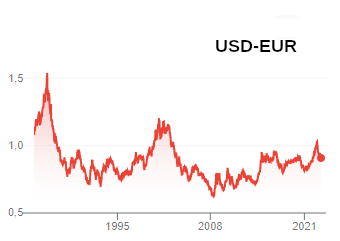
\includegraphics[width=0.9\linewidth]{usd_eur}
    	\column{0.5\linewidth}
      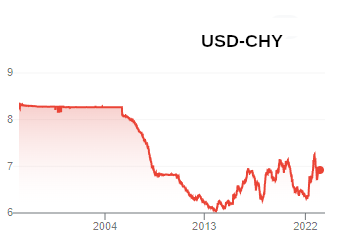
\includegraphics[width=0.9\linewidth]{usd_chy}
    \end{columns}
  \end{itemize}
\end{frame}

\begin{frame}{Numeraires}
  \begin{itemize}
  \item Of course, in practice there are reasons to prefer gold to other commodities e.g. corn, live cattle, or one currency with respect to another (i.e. political reasons)\ldots
  \item But intuitively there should be no theoretical reason (at least at the scale of investors) to measure value in gold or USD (there used to be also the ``gold standard'')
  \item Basically we want to exploit this fact in our financial models.
  \end{itemize}
\end{frame}

\begin{frame}{Numeraires}
  \begin{itemize}
  \item<1-> \textcolor{red}{Deterministic numeraires} are easy to handle as they imply just an algebraic transformation (i.e. do not involve any risk),
    \begin{itemize}
    \item the exchange rate of the Italian Lira to the Euro was locked at EUR 1 = ITL 1936.27 on 31 December 1998.
    \end{itemize}
  \item<2-> When the numeraire is a stochastic process, and we want to move to it, the pricing of a claim has to be changed in order to take into account the new risks (the intrinsic randomness of the new numeraire).
  \item<3-> In particular a change of numeraire implies also a change in the measure (probability distribution). Indeed (starting with the bank account numeraire)
    \begin{equation*}
      \begin{cases}
        \cfrac{S_1}{B_t} = \cfrac{\sum_i S^i_1 p_i}{e^{rt}}\\
        \cfrac{S_2}{B_t} = \cfrac{\sum_i S^i_2 p_i}{e^{rt}}
      \end{cases}\implies
      \frac{S_1}{S_2} = \frac{\sum_i S^i_1 p_i}{\sum_j S^j_2 p_j} = \sum_i S_1^i \frac{p_i}{\sum_j S^j_2 p_j} = \sum_i S_1^1 \pi_i
    \end{equation*}
  \end{itemize}
\end{frame}

\begin{frame}{Numeraire Examples (I)}
  \begin{itemize}
  \item<1-> \textbf{Money market account.} Given $r_t$, a possibly random and time dependent risk-free interest rate process, let
    \begin{equation*}
      N_t := \exp\left(\int_0^t r_s ds\right)
    \end{equation*}
    In this case 
    \begin{equation*}
      \tilde{S_t}:=\frac{S_t}{N_t}=e^{-\int_0^t r_s ds}S_t, \quad t \ge 0
    \end{equation*}
    represents the discounted price of the asset at time 0.
  \item<2-> \textbf{Currency exchange rate.} In this case $N_t := R_t$ denotes e.g. the EUR/SGD exchange rate. Let
    \begin{equation*}
      \tilde{S_t}:=\frac{S_t}{R_t}, \quad t \ge 0
    \end{equation*}
    denotes the price of a local (SG) asset quoted in units of the foreign currency (EUR) (notice the difference with previous ITL/EUR example above).
  \end{itemize}
\end{frame}

\begin{frame}{Numeraire Examples (II)}
  \begin{itemize}
  \item<1-> \textbf{Forward numeraire.} The price $P(t,T)$ of a bond paying $P(T,T)=1$ at maturity $T$. In this case
    \begin{equation*}
      N_t := P(t,T)=\mathbb{E}\left[e^{\int_t^T r_s ds}\right]
    \end{equation*}
    %Notice that the process $t\rightarrow e^{\int_0^t r_s ds} P(t,T)=\mathbb{E}\left[e^{\int_0^T r_s ds}\right], \quad 0 \le t \le T$ is a martingale.
  \item<2-> \textbf{Annuity numeraire.} Processes of the form
    \begin{equation*}
      N_t = P(t, T_0, T_n) := \sum_{k=1}^{n}(T_k - T_{k-1})P(t, T_k), \quad 0 \le t \le T
    \end{equation*}
    where $P(t,T_1),P(t,T_2),\ldots,P(t,T_n)$ are bond prices with maturities $T_1 < T_2 < \ldots < T_n$.
  \end{itemize}
\end{frame}

\subsection{Radon-Nikodym Derivative}
\begin{frame}{Radon-Nikodym Derivative}
  \begin{itemize}
  \item Now we need to understand how to pass from a numeraire to another, and hence by a measure to another, in an arbitrage free setting.
  \item Notice that until now we have implicitly assumed the bank account $B$ as numeraire.
  \end{itemize}
	\pause
  \begin{block}{Definition}
    When two measures are equivalent it is possible to express the first in terms of the second through the \textcolor{red}{Radon-Nikodym derivative}. Indeed there exists a \textcolor{red}{martingale process $\zeta_t$} such that
    \begin{equation*}
      \mathcal{Q}^* =\int_{A} \zeta_t(\omega)d\mathcal{Q}(\omega)
    \end{equation*}
    which can be written in a more concise form as
    \begin{equation}
      \frac{d\mathcal{Q}^*}{d\mathcal{Q}} = \zeta_t
      \label{eq:radon_nikodym_der}
    \end{equation}
  \end{block}
\end{frame}

\begin{frame}{Intuition from Expected Value}
  \begin{itemize}
  \item To get a sense of what a Radon-Nikodym derivative is we can write the expected value of a generic function $\Pi(x)$ under a measure $\mathcal{F}$, with associated density function $f(x)$ as
    \begin{equation*}
      \mathbb{E}^\mathcal{F}=\int\Pi(x)f(x)dx
    \end{equation*}
  \item Suppose there exists a function $g(x)$, which satisfies the mathematical conditions required to be a density function. Then we can write
    \begin{equation*}
      \mathbb{E}^\mathcal{F}=\int\Pi(x)f(x)\frac{g(x)}{g(x)}dx
    \end{equation*}
  \item If we define $\psi(x)=\Pi(x)\frac{f(x)}{g(x)}$ the expected value can be written as 
    \begin{equation*}
      \mathbb{E}^\mathcal{F}[\Pi(x)]=\int\psi(x)g(x)dx=\mathbb{E}^\mathcal{G}[\psi(x)]=\mathbb{E}^\mathcal{G}\left[\Pi(x)\frac{f(x)}{g(x)}\right]
    \end{equation*}
  \end{itemize}
\end{frame}

\begin{frame}{Radon-Nikodym Derivative}
  \begin{itemize}
  \item The expectations corresponding to the two measures are related by
    \begin{equation*}
      \mathbb{E}^{\mathcal{Q}^*}[X] = \mathbb{E}^\mathcal{Q}\left[X\frac{d\mathcal{Q}^*}{d\mathcal{Q}}\right]
    \end{equation*}
	\pause
  \item In case of a conditioned expectation
    \begin{equation}
      \mathbb{E}^*[X|\mathcal{F}_t] = \frac{\mathbb{E}\left[X\cfrac{d\mathcal{Q}^*}{d\mathcal{Q}}\bigg|\mathcal{F}_t\right]}{\mathbb{E}[\zeta_t|\mathcal{F}_t]}
      \label{eq:conditioned_expectation}
    \end{equation}
    which is an "equivalent" formulation of the famous \emph{Bayes theorem}
    \begin{equation*}
      P(A|B)=\frac{P(B|A)P(A)}{P(B)}
    \end{equation*}
  \end{itemize}
\end{frame}

\subsection{Change of Numeraire}
\begin{frame}{Change of Numeraire}
  \begin{block}{Theorem}
    Assume exists a numeraire $N_t$ and the associated measure $\mathcal{Q}^N$, equivalent to $\mathcal{P}$, such that the price of any traded asset $S_t$ relative to $N$ is a martingale under $\mathcal{Q}^N$
    \begin{equation*}
      \frac{S_t}{N_t} = \mathbb{E}^N\left[\frac{S_T}{N_T}\bigg|\mathcal{F}_t\right],\quad 0\le t \le T
    \end{equation*}
    Let $U$ be another arbitrary numeraire. Then there exists a measure $\mathcal{Q}^U$, also equivalent to $\mathcal{P}$, such that the price of any traded asset $S_t$, normalized to $U$, is a martingale under $\mathcal{Q}^U$
    \begin{equation*}
      \frac{S_t}{U_t} = \mathbb{E}^U\left[\frac{S_T}{U_T}\bigg|\mathcal{F}_t\right],\quad 0\le t \le T
    \end{equation*}
  \end{block}
\end{frame}	

\begin{frame}{Change of Numeraire}
  \begin{block}{...continued}
    The Radon-Nikodym derivative defining the measure $\mathcal{Q}^U$ is given by
    \begin{equation}
      \frac{d\mathcal{Q}^U}{d\mathcal{Q}^N} = \frac{U_T N_0}{U_0 N_T}
      \label{eq:radon_nikodym_der2}
    \end{equation}
  \end{block}
\end{frame}

\begin{frame}{Change of Numeraire (Proof p.2)}
  Let's prove first this second part.
  By definition of $\mathcal{Q}^N$, for any asset price $S_t$ holds
  \begin{equation*}
    \begin{cases}
      \cfrac{S_0}{N_0} = 
      \mathbb{E}^N\left[\cfrac{S_T}{N_T}\right] \\
      \cfrac{U_0}{N_0}\mathbb{E}^U\left[\cfrac{S_T}{U_T}\right] = \cfrac{\cancel{U_0} S_0}{N_0 \cancel{U_0}} = \cfrac{S_0}{N_0}
    \end{cases}\implies \mathbb{E}^N\left[\frac{S_T}{N_T}\right] = \mathbb{E}^U\left[\frac{U_0 S_T}{N_0 U_T}\right]
  \end{equation*}
  since both equal $S_0/N_0$. 
\end{frame}

\begin{frame}{Change of Numeraire (Proof p.2)}
  Also, by definition of Radon-Nikodym derivative
  \begin{equation*}
    \mathbb{E}^N\left[\frac{S_T}{N_T}\right] = \mathbb{E}^U\left[\frac{S_T}{N_T} \frac{d\mathcal{Q}^N}{d\mathcal{Q}^U}\right]
  \end{equation*}
	\pause
  But from the previous result
  \begin{equation*}
    \mathbb{E}^N\left[\frac{S_T}{N_T}\right] = \mathbb{E}^U\left[\frac{U_0 S_T}{N_0 U_T}\right]
  \end{equation*}
  The expectation arguments under $U$ must equal, so we get \cref{eq:radon_nikodym_der2}. 
  \pause
  
  This last equation shows that \textcolor{red}{the risk-neutral price is invariant under change of numeraire.}
    \begin{equation*}
    Price_0 = \mathbb{E}^N\left[\frac{N_0 S_T}{N_T}\right] = \mathbb{E}^U\left[\frac{U_0 S_T}{U_T}\right]
  \end{equation*}
  
\end{frame}

\begin{frame}{Change of Numeraire (Proof p.1)}
  \begin{itemize}
  \item<1-> Now we can prove the first part of the change of numeraire theorem. The conditional expectation formula~\cref{eq:conditioned_expectation} gives
    \begin{equation*}
      \mathbb{E}^U\left[\cfrac{S_T}{U_T}\bigg|\mathcal{F}_t\right]=\cfrac{\mathbb{E}^N\left[\cfrac{d\mathcal{Q}^U}{d\mathcal{Q}^N}\cfrac{S_T}{U_T}\bigg|\mathcal{F}_t\right]}{\mathbb{E}^N\left[\cfrac{d\mathcal{Q}^U}{d\mathcal{Q}^N}\bigg|\mathcal{F}_t\right]}
    \end{equation*}
  \item<2-> But 
    \begin{equation*}
      \begin{cases}
	\mathbb{E}^N\left[\cfrac{d\mathcal{Q}^U}{d\mathcal{Q}^N}\cfrac{S_T}{U_T}\bigg|\mathcal{F}_t\right]= \mathbb{E}^N\left[\cfrac{\cancel{U_T} N_0}{N_T U_0}\cfrac{S_T}{\cancel{U_T}}\bigg|\mathcal{F}_t\right]=\cfrac{N_0 S_t}{U_0 N_t} \\
	\mathbb{E}^N\left[\cfrac{d\mathcal{Q}^U}{d\mathcal{Q}^N}\bigg|\mathcal{F}_t\right]= \mathbb{E}^N\left[\cfrac{U_T N_0}{N_T U_0}\bigg|\mathcal{F}_t\right] = \cfrac{N_0 U_t}{U_0 N_t}
      \end{cases}\implies
      \frac{S_t}{\cancel{N_t}}=\mathbb{E}^U\left[\cfrac{S_T}{U_T}\bigg|\mathcal{F}_t\right]\frac{U_t}{\cancel{N_t}}
    \end{equation*}
  \end{itemize}
\end{frame}	

\begin{frame}{Change of Numeraire Remarks}
  \begin{itemize}
  \item The powerful theorem we have just proved allows to
    \begin{itemize}
    \item find a characterization of our process by means of which we can work-out more easily the fundamental pricing formula. In particular allows to find a measure associated to the new numeraire such that \textcolor{red}{the price of any asset divided by that numeraire is a martingale};
    \item give a simple rule to write (the otherwise difficult to derive) Radon-Nikodym derivative;
    \item show that \textcolor{red}{the risk-neutral price is invariant under change of numeraire.}
    \end{itemize}
  \end{itemize}
\end{frame}

\begin{frame}{Asset Price divided by Numeraire}
	\begin{itemize}
 	\item<1-> Let $B$ be the money bank numeraire and $\mathcal{Q}^B$ the corresponding risk-neutral measure. Also let $N$ be another numeraire (note that $N/B$ is a $\mathcal{Q}^B$-martingale). 
	\item<2-> From the Change of Numeraire Theorem we can define a new measure by mean of
  \begin{equation*}
    \frac{d\mathcal{Q}^N}{d\mathcal{Q}^B} = \frac{N_TB_0}{B_TN_0}
  \end{equation*}
	\item<3-> Then, for any asset $S$ such that $S/B$ is a $\mathcal{Q}^B$-martingale
  \begin{equation*}
    \mathbb{E}^N\left[\frac{S_T}{N_T}\bigg|\mathcal{F}_t\right] = \cfrac{\mathbb{E}^B\left[\cfrac{S_T}{N_T}\cfrac{N_TB_0}{B_TN_0}\bigg|\mathcal{F}_t\right]}{\mathbb{E}^B\left[\cfrac{N_TB_0}{B_TN_0}\bigg|\mathcal{F}_t\right]}
    =\cfrac{\mathbb{E}^B\left[\cfrac{S_T}{B_T}\bigg|\mathcal{F}_t\right]}
    {\mathbb{E}^B\left[\cfrac{N_T}{B_T}\bigg|\mathcal{F}_t\right]}
    =\frac{S_tB_t}{N_tB_t}=\frac{S_t}{N_t}
  \end{equation*}
	\item<4-> \textcolor{red}{So $S/N$ is a $\mathcal{Q}^N$-martingale.}
	\end{itemize}
\end{frame}

\subsection{Applications}
\begin{frame}{Examples}
  \footnotesize{\tiny {\tiny }}{
    \begin{table}[bt]
      \renewcommand*{\arraystretch}{1.4}
      \begin{tabular}{|l|l|} \hline
	\begin{tabular}{@{}l@{}}
	  Any asset divided by the bank account
	  $B_t$\\(recall $dB_t = r_t B_t dt$)
	  \boxed{\cfrac{S_t}{B_t} = e^{-\int_0^t r_s ds}S_t}
	\end{tabular}
	& \begin{tabular}{l}
	    It is a martingale under the\\
	    measure $Q^B$ associated to \\
	    the bank account numeraire,\\
  	    i.e. the risk neutral measure.
	  \end{tabular} \\ \hline
	\begin{tabular}{@{}l@{}}
	  The forward rate\\
	  \boxed{F(t; T_1, T_2) = \frac{1}{T_2-T_1}\left(\frac{P(t,T_1) - P(t,T_2)}{P(t,T_2)}\right)}\\
	  can be interpreted as a portfolio of two ZCBs\\
	  divided by another ZCB.		
	\end{tabular}
	& \begin{tabular}{l}
	    Under the measure $\mathcal{Q}^2$\\ 
	    associated to the numeraire\\ 
	    $P(\cdot,T_2)$ it is a martingale.\end{tabular}\\ \hline  
	\begin{tabular}{@{}l@{}}
	  The swap rate
	  \boxed{S_{\alpha,\beta}(t) = \frac{P(t,T_\alpha)-P(t,T_\beta)}{\sum_{i=\alpha+1}^{\beta}\tau_i P(t,T_i)}}
	  \\can be interpreted as a portfolio of two ZCBs\\
	  divided by a portfolio of ZCBs.		
	\end{tabular}
	& \begin{tabular}{l}
	    It is a martingale under the\\
	    measure associated to the\\
	    annuity numeraire.
	  \end{tabular} \\ \hline
      \end{tabular}
  \end{table}}
\end{frame}

\begin{frame}{A Useful Separation}
  \begin{itemize}
  \item<1-> Until now we have used $B(t)$, the money market account, as numeraire. But as we have seen it is natural to look for the most convenient numeraire, which minimizes the mathematical difficulties according to the problem at hand.
  \item<2-> Given a contingent claim whose payoff at time $T$ is $\chi$, we have the following formula for its price $\Pi$
    \begin{equation*}
      \Pi_\chi(t,T)=\mathbb{E}^B\left[e^{-\int_t^T r_s ds}\chi\bigg|\mathcal{F}_t \right]=\mathbb{E}^B\left[e^{\int_0^t r_s ds}e^{-\int_0^T r_s ds}\chi\bigg|\mathcal{F}_t \right]=B_t\mathbb{E}^B\left[B^{-1}_T\chi|\mathcal{F}_t\right]
    \end{equation*}
  \item<3-> If $\chi$ and the short rate process were independent under $\mathcal{Q}^B$ (recall $\mathbb{E}[XY]=\mathbb{E}[X]\mathbb{E}[Y]$) then we could write
    \begin{equation*}
      \Pi_\chi(t,T)=\mathbb{E}^B\left[e^{-\int_t^T r_s ds}\bigg|\mathcal{F}_t\right]\mathbb{E}^B\left[\chi|\mathcal{F}_t\right] = P(t,T)\mathbb{E}^B\left[\chi|\mathcal{F}_t\right]
    \end{equation*}
  \end{itemize}
\end{frame}

\begin{frame}{A Useful Separation}
  \begin{itemize}
  \item<1-> In general the above separation is not possible due to the interaction between the discount factors and the claim payoff. 
  \item<2-> In this, like in other concrete situations, a better numeraire is indeed the ZCB with the same maturity $T$ of the derivative to price (recall $P(T,T)=1)$.
  \item<3-> The \textcolor{red}{forward measure $\mathcal{Q}^T$ (also called the $T$-measure)} is defined as the martingale measure for the numeraire process $P(\cdot,T)$, the ZCB maturing in T indeed, i.e. what we called $\mathcal{Q}^2$ in the example above.
  \item<4-> It is easy to see that using \cref{eq:radon_nikodym_der2}, the Radon-Nykodim derivative is given in this case by
    \begin{equation}
      \zeta_t = \frac{d\mathcal{Q}^T}{d\mathcal{Q}^B} = \frac{P(t,T)\overbrace{B(0)}^{=1}}{B_t P(0,T)} ,\quad\left(\zeta_T=\frac{\overbrace{P(T,T)}^{=1}B(0)}{B(T)P(0,T)}=\frac{1}{B(T)P(0,T)}\right)
      \label{eq:radon_nikodym_t_forward}
    \end{equation}
  \end{itemize}
\end{frame}

\begin{frame}{A Useful Separation}
  \begin{itemize}
  \item<1-> Applying the change of numeraire to the pricing formula, we get
    \begin{equation*}
      \begin{aligned}
	\Pi_\chi(t,T) & = B_t\mathbb{E}^B\left[B^{-1}_T\chi|\mathcal{F}_t\right] \\
	& = B_t\mathbb{E}^B\left[P(0,T)\zeta_T\chi|\mathcal{F}_t\right]\quad\text{(using } B_T^{-1} = \zeta_TP(0,T))\\
	& = B_tP(0,T)\mathbb{E}^B\left[\zeta_T|\mathcal{F}_t\right]\mathbb{E}^T\left[\chi|\mathcal{F}_t\right]\quad\text{(by \cref{eq:conditioned_expectation})}\\
	& = \cancel{B_tP(0,T)}\frac{P(t,T)}{\cancel{B_tP(0,T)}}\mathbb{E}^T\left[\chi|\mathcal{F}_t\right] \\
	& = P(t,T)\mathbb{E}^T\left[\chi|\mathcal{F}_t\right] \\
      \end{aligned}
    \end{equation*}
    which achieves the desired separation (although under a new measure).
  \item<2-> Clearly this kind of transformation is useful when $\chi$ has known dynamics under the forward measure.
  \end{itemize}
\end{frame}

\begin{frame}{Identity between $\mathcal{Q}^B$ and $\mathcal{Q}^T$}
  By construction of the martingale measure $\mathcal{Q}^B$, the following relationship holds
  \begin{equation*}
    \begin{gathered}
      \frac{P(t,T)}{B_t}=\mathbb{E}^B\left[\frac{P(T,T)}{B_T}\right]\\[0.3cm]
      P(t,T)=\mathbb{E}^B\left[\frac{P(T,T)}{B_T}B_t\right] = \mathbb{E}^B\left[\frac{B_t}{B_T}\right]
    \end{gathered}
  \end{equation*}
	\pause
  Plugging the result into the Radon-Nikodym derivative gives
  \begin{equation*}
    \frac{d\mathcal{Q}^T}{d\mathcal{Q}^B} = \frac{B_t}{B_T}\frac{1}{P(t,T)} =\frac{B_t/B_T}{\mathbb{E}^B[B_t/B_T]}
  \end{equation*}
	\pause
  \begin{block}{Proposition}
    If interest rates are deterministic (i.e. the Radon-Nikodym derivative is 1), then the measures $\mathcal{Q}^B$ and $\mathcal{Q}^T$ are identical.
  \end{block}
\end{frame}

\begin{frame}{Clarification on Time}
  \begin{itemize}
  \item Clearly as the Radon-Nikodym derivative is a martingale for valuation time $t$, we have
    \begin{equation*}
      \frac{d\mathcal{Q}^U}{d\mathcal{Q}^N}=\frac{U_tN_0}{U_0N_t}
    \end{equation*}
  \item Do not confuse the maturity of the numeraire bond $T$ with the times at which you have to take the values of the numeraire, in this case $t$ and 0.
  \item If you want to switch from the $T$ measure to the $S$ measure, i.e. the one induced by the bond $P(.,S)$, for the valuation time $t$ we get
    \begin{equation*}
      \frac{d\mathcal{Q}^S}{d\mathcal{Q}^T}=\frac{P(t,S)P(0,T)}{P(t,T)P(0,S)}
    \end{equation*}
  \end{itemize}
\end{frame}

\begin{frame}{The Forward Rate Under $\mathcal{Q}^T$}
  \begin{block}{Proposition}
    Consider the forward numeraire $P(t,T)$ and denote with $\mathcal{Q}^T$ its associated measure.
    The forward rate spanning the interval $[S,T]$ is the $\mathcal{Q}^T$-expectation of the future spot rate at time $S$ for the maturity $T$
    \begin{equation}
      F(t;S,T) =\mathbb{E}^T[L(S,T)|\mathcal{F}_t]
    \end{equation}
  \end{block}
\end{frame}

\begin{frame}{The Forward Rate Under $\mathcal{Q}^T$ (Proof)}
  \begin{equation*}
    \begin{gathered}
      F(t;S,T) = \frac{1}{\tau}\left[\frac{P(t,S)-P(t,T)}{P(t,T)}\right] \\[0.3cm]
      F(t;S,T)P(t,T) = \frac{P(t,S)-P(t,T)}{\tau}
    \end{gathered}
  \end{equation*}

  This is the price at time $t$ of an asset (difference of two bonds). Therefore by the change of numeraire theorem and by definition of forward measure
  \begin{equation*}
    \frac{F(t;S,T)P(t,T)}{P(t,T)} = F(t,S,T)
  \end{equation*}
  is a \textcolor{red}{martingale} under $\mathcal{Q}^T$-measure. \pause Hence
  \begin{equation*}
    F(t;S,T) = \mathbb{E}^T[F(S;S,T)|\mathcal{F}_t] = \mathbb{E}^T\left[\frac{1}{\tau}\left(\frac{1-P(S,T)}{P(S,T)}\right)\bigg|\mathcal{F}_t\right] = \mathbb{E}^T[L(S,T)|\mathcal{F}_t]
  \end{equation*}
\end{frame}

\begin{frame}{The Forward Rate Under $\mathcal{Q}^T$}
  A similar result can be derived for the corresponding instantaneous quantities
  \begin{equation}
    f(t,T)=\mathbb{E}^T[r_t|\mathcal{F}_t]
  \end{equation}
	\pause
  Indeed from the definition of $\mathcal{Q}^B$
  \begin{equation*}
    \frac{P(t,T)}{B_t}=\mathbb{E}^B\left[\frac{P(T,T)}{B_T}\bigg|\mathcal{F}_t\right]
  \end{equation*}
  but $P(T,T)=1$ so
  \begin{equation*}
    P(t,T)=\mathbb{E}^B\left[\frac{B_tP(T,T)}{B_T}\bigg|\mathcal{F}_t\right]=\mathbb{E}^B\left[e^{-\int_t^Tr_u du}\big|\mathcal{F}_t\right]
  \end{equation*}
	\pause
  Differentiating with respect to $T$ ($\frac{d}{dx}\int_c^x f(t)dt=f(x)$)
  \begin{equation*}
    \frac{\partial P(t,T)}{\partial T}=
    \mathbb{E}^B\left[-r(T)e^{-\int_t^Tr_u du}\big|\mathcal{F}_t\right]
  \end{equation*}
\end{frame}

\begin{frame}{The Forward Rate Under $\mathcal{Q}^T$}
  Now we can change numeraire to $P(\cdot,T)$ so that, using reciprocal of \cref{eq:radon_nikodym_t_forward} ($\zeta^{-1}=\frac{B_t/B_T}{P(t,T)/P(T,T)}$)
  \begin{equation*}
    \frac{\partial P(t,T)}{\partial T}=
    \mathbb{E}^T\left[-r(T)\cancel{e^{-\int_t^Tr_u du}}\frac{P(t,T)}{\cancel{e^{-\int_t^Tr_u du}}}\bigg|\mathcal{F}_t\right]=
    P(t,T)\mathbb{E}^T\left[-r(T)|\mathcal{F}_t\right]
  \end{equation*}
	\pause
  Hence
  \begin{equation*}
    \begin{aligned}
      f(t,T)&=\frac{1}{P(t,T)}\frac{\partial P(t,T)}{\partial T}=
      -\frac{\partial \ln P(t,T)}{\partial T}
      = \mathbb{E}^T\left[r(T)|\mathcal{F}_t\right]=	\mathbb{E}^T\left[f(T,T)|\mathcal{F}_t\right]
    \end{aligned}
  \end{equation*}
  Which demonstrates the initial statement and also shows that \textcolor{red}{the instantaneous forward rate is a martingale under the $T$-forward measure}.
\end{frame}

\begin{frame}{The Expectation Hypothesis}
	\begin{itemize}
		\item Previous result
		\begin{equation*}
			f(t, T) = \mathbb{E}^T[r(T)|\mathcal{F}_t]
		\end{equation*}
		has a nice connection with the \textcolor{red}{expectation hypothesis of the term structure of interest rates}.
		\item Its basic idea is that the long-term rate is determined purely by current and future expected short-term rates.
		\item We cannot dive into it, but there are tons of papers on the subject, among which I suggest
		\begin{itemize}
			\item \href{https://pages.stern.nyu.edu/~sternfin/asangvin/ExpHyp.pdf}{\emph{The Expectation Hypothesis, A. Sangvinatsos}}
			\item \href{https://www.jstor.org/stable/2327547}{\emph{A Re-Examination of Traditional Hypotheses about the Term Structure of Interest Rates}, J.C. Cox, J.E. Ingersoll, and S.A. Ross}
			%\item \href{https://www.albany.edu/~bd445/Economics_802_Financial_Economics_Slides_Fall_2013/Risk_Neutrality_and_the_Expectations_Theory.pdf}{\emph{Slides from Fall 2013}}
		\end{itemize}
	%\item According to the pure expectation hypothesis, the above formula is valid if the expected value is taken under the real probability.
	%\item Absence of arbitrage makes this incompatible with stochastic interest rates.
	\end{itemize}
\end{frame}

%The Relationship between Forward Rate over Second Year
%and Spot Rate Expected over Second Year
%Given a forecast of bond B’s price, an investor can choose one of two strategies at date 0:
% 1. Buy a one-year bond. Proceeds at date 1 would be:
% $1,080 = $1,000 x 1.08 (A.10)

% 2. Buy a two-year bond but sell at date 1. Expected proceeds would be:
% $1,000 x (1.10)2
%____________________________
%1 +  Spot rate expected over year 2 (A.11)
% Given our discussion of forward rates, we can rewrite Equation A.11 as:
% $1,000 x 1.08 x 1.1204
%____________________________
%1  Spot rate expected over year 2 (A.12)
% (Remember that 12.04 percent was the forward rate over year 2; that is, f2 = 12.04%.)
% Under what condition will the return from strategy 1 equal the expected return from
%strategy 2? In other words, under what condition will Equation A.10 equal Equation A.12?
% The two strategies will yield the same expected return only when:
% 12.04%  Spot rate expected over year 2 (A.13)
%In other words, if the forward rate equals the expected spot rate, one would expect to earn
%the same return over the first year whether one
%• Invested in a one-year bond.
%• Invested in a two-year bond but sold after one year.


%The Expectations Hypothesis
%Equation A.13 seems fairly reasonable. That is, it is reasonable that investors would set
%interest rates in such a way that the forward rate would equal the spot rate expected by the
%marketplace a year from now.
% For example, imagine that individuals in the marketplace do
%not concern themselves with risk. If the forward rate, f2, is less than the spot rate expected
%over year 2, individuals desiring to invest for one year would always buy a one-year bond.
%That is, our work shows that an individual investing in a two-year bond but planning to sell
%at the end of one year would expect to earn less than if he simply bought a one-year bond.
% Equation A.13 was stated for the specific case where the forward rate was 12.04 percent.
%We can generalize this as follows:
%Expectations Hypothesis:
% f2 = Spot rate expected over year 2 (A.14)
%Equation A.14 says that the forward rate over the second year is set to the spot rate that
%people expect to prevail over the second year. This is called the expectations hypothesis. It
%states that investors will set interest rates such that the forward rate over the second year is
%equal to the one-year spot rate expected over the second year.


%Liquidity Preference Hypothesis
%At this point, many students think that Equation A.14 must hold. However, note that we
%developed Equation A.14 by assuming that investors were risk-neutral. Suppose, alternatively, that investors are averse to risk.
% Which strategy would appear more risky for an individual who wants to invest for one year?
% 1. Invest in a one-year bond.
% 2. Invest in a two-year bond but sell at the end of one year.

%Strategy 1 has no risk because the investor knows that the rate of return must be r1. Conversely,
%strategy 2 has much risk: The fi nal return is dependent on what happens to interest rates.
% Because strategy 2 has more risk than strategy 1, no risk-averse investor will choose
%strategy 2 if both strategies have the same expected return. Risk-averse investors can have
%no preference for one strategy over the other only when the expected return on strategy
%2 is above the return on strategy 1. Because the two strategies have the same expected
%return when f2 equals the spot rate expected over year 2, strategy 2 can have a higher rate
%of return only when the following condition holds:
%Liquidity Preference Hypothesis:
% f2 >  Spot rate expected over year 2 (A.15)

%That is, to induce investors to hold the riskier two-year bonds, the market sets the forward
%rate over the second year to be above the spot rate expected over the second year. Equation A.15 is called the liquidity preference hypothesis.
% We developed the entire discussion by assuming that individuals are planning to invest
%over one year. We pointed out that for these types of individuals, a two-year bond has extra
%risk because it must be sold prematurely. What about individuals who want to invest for two
%years? (We call these people investors with a two-year time horizon.)
% They could choose one of the following strategies:
% 3. Buy a two-year zero coupon bond.
% 4. Buy a one-year bond. When the bond matures, immediately buy another one-year bond.
% Strategy 3 has no risk for an investor with a two-year time horizon because the proceeds
%to be received at date 2 are known as of date 0. However, strategy 4 has risk because the
%spot rate over year 2 is unknown at date 0. It can be shown that risk-averse investors will
%prefer neither strategy 3 nor strategy 4 over the other when:
% f2 < Spot rate expected over year 2 (A.16)

% Note that the assumption of risk aversion gives contrary predictions. Relationship A.15
%holds for a market dominated by investors with a one-year time horizon. Relationship A.16
%holds for a market dominated by investors with a two-year time horizon. Financial economists have generally argued that the time horizon of the typical investor is generally much
%shorter than the maturity of typical bonds in the marketplace. Thus, economists view A.15
%as the best depiction of equilibrium in the bond market with risk-averse investors.
% However, do we have a market of risk-neutral or risk-averse investors? In other words,
%can the expectations hypothesis of Equation A.14 or the liquidity preference hypothesis of
%Equation A.15 be expected to hold? As we will learn later in this book, economists view
%investors as being risk-averse for the most part. Yet, economists are never satisfi ed with a
% casual examination of a theory’s assumptions. To them, empirical evidence of a theory’s
%predictions must be the fi nal arbiter.
% There has been a great deal of empirical evidence about the term structure of interest
%rates. Unfortunately (perhaps fortunately for some students), we will not be able to present
%the evidence in any detail. Suffi ce it to say that, in our opinion, the evidence supports the
% liquidity preference hypothesis over the expectations hypothesis. One simple result might
%give students the fl avor of this research. Consider an individual choosing between one of
%the following two strategies:
% 1. Invest in a one-year bond.
% 2. Invest in a 20-year bond but sell at the end of one year.
%www.mhhe.com/rwj r
%Chapter 5 How to Value Bonds and Stocks 5A-9
% [Strategy 2 is identical to strategy 2, except that a 20-year bond is substituted for a
%2-year bond.]
% The expectations hypothesis states that the expected returns on both strategies are
%iden tical. The liquidity preference hypothesis states that the expected return on strategy
%2 should be above the expected return on strategy 1. Though no one knows what returns
%are actually expected over a particular time period, actual returns from the past may allow
%us to infer expectations. The results from January 1926 to December 1999 are illuminating. The average yearly return on strategy 1 is 3.8 percent and 5.5 percent on strategy 2
%over this time period.7,8 This evidence is generally considered to be consistent with the
% liquidity preference hypothesis and inconsistent with the expectations hypothesis.
%\end{frame}

\subsection{Girsanov Theorem}
\begin{frame}{Which Dynamics ?}
  \begin{itemize}
  \item<1-> We're left with one important question:
    \textcolor{red}{what does the path of an asset price $S_t$ look like under a new measure $\mathcal{Q}$ ?} (we need to know in order to be able to really compute its expectation under $\mathcal{Q}$.)
  \item<2-> \emph{Girsanov's theorem} answers to this question since it tells us, when we change from $\mathcal{P}$ to some other measure $\mathcal{Q}$, how the stochastic part of a process ($W_t$) changes under $\mathcal{Q}$.
  \item<3-> Will see that it evolves as the sum of a Brownian motion under $\mathcal{Q}$ and a drift related to the Radon-Nikodym derivative characterizing $\mathcal{Q}$.
  \item<4-> We therefore want to choose the Radon-Nikodym derivative so that the drift of $W_t$ w.r.t. $\mathcal{Q}$ exactly cancels out the drift of $S_t$, leaving us with a pure diffusion process (martingale). 
  \end{itemize}
\end{frame}

\begin{frame}{Girsanov Theorem}
  \begin{block}{Theorem}
    Consider the SDE 
    \begin{equation*}
      dX_t = f_t dt + \sigma_t dW_t
    \end{equation*}
    under $\mathcal{P}$. 
    
    Let be given a new drift $f^*_t$ and assume $\gamma_t=\frac{f_t^*-f_t}{\sigma_t}$ such that $\mathbb{E}\left[\exp\left(\frac{1}{2}\int_0^t\gamma_t^2dt\right)\right]<\infty$.
    Define the measure 
    \begin{equation}
      \frac{d\mathcal{P}^*}{d\mathcal{P}}=\exp\left(-\frac{1}{2}\int_0^t \gamma_s^2 ds + \int_0^t \gamma_s dW_s \right)
    \end{equation}
    Then $\mathcal{P}^*$ is equivalent to $\mathcal{P}$. 
    The Radon-Nikodym derivative process is an \textcolor{red}{exponential martingale}.
  \end{block}
\end{frame}

\begin{frame}{Girsanov Theorem}
  \begin{block}{Theorem continued}
    Also the process
    \begin{equation}
      dW^*_t = -\gamma_s dt + dW_t
    \end{equation} 
    is a Brownian motion under $\mathcal{P}^*$, and 
    \begin{equation*}
      dX_t = f^*_t dt + \sigma_t dW^*_t
    \end{equation*}
    The condition $\mathbb{E}\left[\exp\left(\frac{1}{2}\int_0^t\gamma_t^2dt\right)\right]<\infty$ is a sufficient but non-necessary, and it is know as the \textcolor{red}{Novikov condition}.
  \end{block}
\end{frame}

%\begin{frame}{Girsanov Theorem (Proof)}
%  \begin{itemize}
%  \item We have already seen that the solution of the SDE $dS_t=\mu S_t dt + \sigma S_t dW_t$ is
%    \begin{equation*}
%      \frac{S_t}{S_0} = e^{(\mu-\frac{1}{2}\sigma^2)t+\sigma W_t}
%    \end{equation*}
%  \item If we now assume the drift coefficient $\mu=0$ the solution becomes
%    \begin{equation*}
%      \frac{S_t}{S_0} = e^{(-\frac{1}{2}\sigma^2)t+\sigma W_t} \approxeq \frac{d\mathcal{P}^*}{d\mathcal{P}}
%    \end{equation*}
%  \item So the Radom-Nikodym is a solution of a driftless process hence is a martingale.
%  \end{itemize}
%\end{frame}

\begin{frame}{An Example}
  \begin{itemize}
  \item Consider the stochastic differential equation
    \begin{equation*}
      dX_t = b(X_t, t) dt + a(X_t, t) dW_t
    \end{equation*}
  \item Let's assume that the drift and diffusion coefficients are such that there exists a unique solution to the equation which is $X$.
  \item We want to find a probability measure $\mathcal{P}^*$ such that the drift of $X$ is $\tilde{b}(X_t,t)$ instead of $b(X_t,t)$.
  \end{itemize}
\end{frame}

\begin{frame}{An Example}
  \begin{equation*}
    \begin{aligned}
      dX_t &= \tilde{b}(X_t,t) dt+b(X_t,t) dt -\tilde{b}(X_t,t) dt + a(X_t,t) dW_t = \\
      &=\tilde{b_t} dt + (b_t -\tilde{b_t})dt + a(X_t,t) dW_t =\\
      &=\tilde{b_t}dt+ a_t\overbrace{\left(\frac{b_t-\tilde{b_t}}{a_t}\right)}^{-\gamma_t}dt + a_t dW_t = \\
      &= \tilde{b_t}dt+a_t dW_t - a_t\gamma_t dt\\
      &=\tilde{b_t}dt+a_t d\tilde{W_t}
    \end{aligned}
  \end{equation*}
  where $d\tilde{W_t}=dW_t-\gamma_t dt$.
\end{frame}

\begin{frame}{An Example}
  \begin{itemize}
  \item<1-> If the Novikov condition is satisfied then we can apply the Girsanov theorem and we have that
    \begin{equation}
      \mathcal{P}^* = \mathbb{E}^\mathcal{P}\left[\exp\left(-\frac{1}{2}\int_0^t \gamma_s^2 ds + \int_0^t \gamma_s dW_s \right)\right]
    \end{equation}
    and that $\tilde{W}$ is a Brownian motion on $\mathcal{P}^*$.
  \item<2-> In practice, don't need to determine the new measure $\mathcal{P}^*$.
  \item<3-> It is enough to know it exists, such that we can work with the resulting SDE of the process of interest under the new measure.	
  \begin{tikzpicture}[remember picture,overlay]
	\node[xshift=5cm,yshift=-3.9cm] (image) at (current page.center) {
\includegraphics[width=20px]{python_logo}};
	\node[align = center, yshift=1.45cm, below=of image] {\tiny{\href{shorturl.at/ctCF7}{shorturl.at/ctCF7}}};
\end{tikzpicture}
  \end{itemize}
\end{frame}

%\begin{frame}{title}
%\begin{itemize}
%	\item Let $(\Omega,\mathcal{F}_t, \mathbb{P})$ be a probability space with a standard Brownian motion $W^{\mathbb{P}}$.
%	\item The stochastic process $S_t$ represents the evolution of a risky security price satisfying stochastic differential equation (SDE)
%	\begin{equation*}
%		dS_t = \mu S_t dt + \sigma S_t dW^{\mathbb{P}}_t
%	\end{equation*}
%	\item Let's assume that interest rate $r$ is constant. Therefore
%	\begin{equation*}
%		D(0,t) = e^{-rt}
%	\end{equation*} 	
%	which implies $dD = -re^{-rtdt}$.  
%\end{itemize}
%\end{frame}
%
%\begin{frame}{title}
%	\begin{itemize}
%		\item Define then 
%		\begin{equation*}
%			Y_t = D_t S_t
%		\end{equation*} 
%		that is the present value at time $t$ of the risky security.
%		\item Using Ito's lemma
%		\begin{equation*}
%			\begin{aligned}
%			dY_t &= D_t dS_t + dD_t S_t \\ 
%			&= D_t (\mu S_t dt + \sigma S_t dW^{\mathbb{P}}_t) + S_t (-rD_t dt) \\
%			&= (\mu - r) Y_t dt + \sigma Y_t dW_t^{\mathbb{P}}		
%			\end{aligned}
%		\end{equation*}
%		\item In its integral form it becomes
%		\begin{equation*}
%			Y_t = Y_0 + (\mu - r)\int_0^t Y_s ds + \sigma \int_0^t Y_s dW_s^{\mathbb{P}}
%		\end{equation*}
%	\end{itemize}
%\end{frame}

%\begin{frame}{Numeraire Pricing}
%	\begin{block}{Theorem (German, El Karoui and Rochet, 1995)}
%		Assume that there exists a numeraire $N$ and a probability measure $\mathcal{Q}^N$ which is equivalent to $\mathcal{P}$ such that, for every traded asset $X$:
%		\begin{equation}
%			\frac{X_t}{N_t} = \mathbb{E}^{\mathcal{Q}^N}\left[\frac{X_T}{N_T}|\mathcal{F}_t\right]
%		\end{equation}
%		Now, given a second arbitrary numeraire $U$, there exists a probability measure $\mathcal{Q}^U$ which is equivalent to $\mathcal{P}$ and such that:
%		\begin{equation}
%			\frac{X_t}{U_t} = \mathbb{E}^{\mathcal{Q}^U}\left[\frac{X_T}{U_T}|\mathcal{F}_t\right]
%		\end{equation}
%	\end{block}
%\end{frame}


%\begin{frame}{Example Approach to Numeraire Change}
%\begin{itemize}
%	\item In lieu of the fundamental theorem we can write
%	\begin{equation}
%	\Pi(0,X)=S_0(0)\mathbb{E}^0\left[\frac{X}{S_0(T)}\right]
%	\end{equation}
%	\item But also
%	\begin{equation}
%	\Pi(0,X)=S_1(0)\mathbb{E}^1\left[\frac{X}{S_1(T)}\right]
%	\end{equation}
%	\item We define the Radon-Nikodym derivative
%	\begin{equation}
%	L_0^1(T)=\frac{dQ^1}{dQ^0}
%	\end{equation}
%\end{itemize}
%\end{frame}
%
%\begin{frame}{Example Approach to Numeraire Change}
%	\begin{itemize}
%		\item Hence we can write ?????????????????
%		\begin{equation}
%			\Pi(0,X)=S_1(0)\mathbb{E}^0\left[\frac{X}{S_1(T)}L_0^1(T)\right]
%		\end{equation}
%		\item After some trivial manipulations
%		\begin{equation}
%			S_0(0)\mathbb{E}^0\left[\frac{X}{S_0(T)}\right]=
%			S_1(0)\mathbb{E}^0\left[\frac{X}{S_1(T)}L_0^1(T)\right]
%		\end{equation}
%		\item Finally
%		\begin{equation}
%			\frac{S_0(0)}{S_0(T)}=\frac{S_1(0)}{S_1(T)}L_0^1(T)		
%		\end{equation}
%	\end{itemize}
%\end{frame}
%
%\begin{frame}{Example Approach to Numeraire Change}
%	\begin{itemize}
%		\item Hence 
%		\begin{equation}
%			L_0^1(T) = \frac{dQ^1}{dQ^0}=			\frac{S_0(0)S_1(0)}{S_1(T)S_0(T)}
%		\end{equation}
%
%	\end{itemize}
%\end{frame}

\begin{frame}{Moving Away from $\mathcal{P}$ Measure}
  \begin{itemize}
  \item<1-> Let's go back to the real-world probabilities and assume that a stock price has the following dynamics (Geometric Brownian Motion) under the real-world measure $\mathcal{P}$
    \begin{equation*}
      dS_t = \mu S_t dt + \sigma S_t dW_t
    \end{equation*}
  \item<2-> By definition the bank account dynamics is described by (for simplicity let's consider deterministic rates)
    \begin{equation*}
      dB_t = rB_tdt\implies B_t = e^{rt}
    \end{equation*}
  \item<3-> We want to know what happens to the stock SDE when moving to two different numeraires:
    \begin{itemize}
    \item<4-> risk-neutral measure (bank account numeraire);
    \item<5-> stock measure (stock numeraire).
    \end{itemize}
  \end{itemize}
\end{frame}

\begin{frame}{Risk-Neutral Measure Dynamics}
  \begin{itemize}
  \item<1-> We have seen that under the bank account induced measure the process defined as an asset divided by the numeraire is a martingale
    \begin{equation*}
      \cfrac{S_t}{B_t} = \mathbb{E}^B\left[\frac{S_T}{B_T}\bigg|\mathcal{F}_t\right]
    \end{equation*}
  \item<2-> So if we define $Z_t=\cfrac{S_t}{B_t}$, since $Z_t$ is a martingale (no-drift process) it's evolution could be described by
    \begin{equation}
      dZ_t = \sigma Z_t dW_t^B
      \label{eq:z_martingale1}
    \end{equation}
    where $dW_t^B$ is a Brownian motion under the $\mathcal{Q}^B$ measure.
  \end{itemize}
\end{frame}

\begin{frame}{Risk-Neutral Measure Dynamics}
  \begin{itemize}
  \item<1-> Computing directly the $Z_t$ differential (by It$\hat{o}$'s rule at first order)
    \begin{equation*}
      \begin{aligned}
	d\left(\frac{S_t}{B_t}\right) &= \frac{dS_t}{B_t} + S_t d\left(\frac{1}{B_t}\right) = \\ 
	&=\frac{dS_t}{B_t} + S_t d\left(e^{-rt}\right) = \frac{dS_t}{B_t} - S_t re^{-rt}dt \\
	&= \frac{dS_t}{B_t} - r\frac{S_t}{B_t}dt 
      \end{aligned}
    \end{equation*}
  \item<2-> Now substitute for $dS_t$
    \begin{equation*}
      d\left(\frac{S_t}{B_t}\right)= \frac{ \mu S_t dt + \sigma S_t dW_t}{B_t} - r\frac{S_t}{B_t}dt = \sigma\frac{S_t}{B_t}\left(\frac{\mu - r}{\sigma}dt + dW_t \right)
    \end{equation*}	
  \end{itemize}
\end{frame}

\begin{frame}{Risk-Neutral Measure Dynamics}
  \begin{itemize}
  \item<1-> In terms of $Z_t$ it becomes
    \begin{equation}
      dZ_t = \sigma Z_t\left(\frac{\mu - r}{\sigma}dt + dW_t \right)
      \label{eq:z_martingale2}
    \end{equation}
  \item<2-> Both \cref{eq:z_martingale2} and~\cref{eq:z_martingale1} represent the dynamics of $Z_t$ so they must be equal
    \begin{equation*}
      \cancel{\sigma Z_t}dW_t^B = \cancel{\sigma Z_t}\left(\frac{\mu - r}{\sigma}dt + dW_t\right)
    \end{equation*}
  \item<3-> Replacing the Brownian Motion into the real-world dynamics
    \begin{equation*}
      \begin{aligned}
	dS_t &= \mu S_t dt + \sigma S_t \left(dW_t^B - \frac{\mu - r}{\sigma}dt\right) =\\
	& = \cancel{\mu S_t dt} \cancel{-\mu S_t dt} + rS_t dt + \sigma S_t dW_t^B  = \boxed{rS_t dt + \sigma S_t dW_t^B}
      \end{aligned}
    \end{equation*}
  \item<4-> So \textcolor{red}{under the risk-neutral measure the drift equals the risk-free rate}.
  \end{itemize}
\end{frame}

\begin{frame}{Stock Numeraire Measure Dynamics}
  \begin{itemize}
  \item<1-> Now let's see what happens under the stock numeraire.
  \item<2-> Under the risk-neutral measure $\mathcal{Q}^B$
    \begin{equation*}
      \frac{S_0}{B_0} = \mathbb{E}^B\left[\frac{S_t}{B_t}\bigg|\mathcal{F}_0\right] \implies
      S_0 = \mathbb{E}^B\left[B_0\frac{S_t}{B_t}\bigg|\mathcal{F}_0\right]
    \end{equation*}
  \item<3-> By the Change of Numeraire Theorem under the measure $\mathcal{Q}^A$ induced by asset numeraire $A$
    \begin{equation*}
      S_0 = \mathbb{E}^A\left[A_0\frac{S_t}{A_t}\bigg|\mathcal{F}_0\right]
    \end{equation*}
  \item<4-> Since both expressions represent a price of an asset they must be the same and we can equal the terms inside the expectations. Note that the expectations are computed according two different measures so we keep the factors $d\mathcal{Q}^X$. 
  \end{itemize}
\end{frame}

\begin{frame}{Stock Numeraire Measure Dynamics}
  \begin{equation*}
    \frac{B_0}{B_t}d\mathcal{Q}^B = \frac{A_0}{A_t}d\mathcal{Q}^A\implies \frac{d\mathcal{Q}^A}{d\mathcal{Q}^B}=\frac{B_0A_t}{B_tA_0}
  \end{equation*}
  \begin{itemize}
  \item<2-> We have already derived the analytical GBM solution in the risk-neutral measure (see pg. 14 to 18 of "no\_arbitrage" slides)
    \begin{equation*} 
      A_t = A_0 \exp\left(rt-\frac{1}{2}\sigma^2 t + \sigma W^B_t\right)
    \end{equation*}
    \item<3-> So we can replace the numeraire definition into the Radon-Nikodym derivative
    \begin{equation*}
      \frac{d\mathcal{Q}^A}{d\mathcal{Q}^B}=\frac{\cancel{A_0}e^{\cancel{rt}-\frac{1}{2}\sigma^2 t + \sigma W^B_t}}{\cancel{e^{rt}}\cancel{A_0}}=\exp\left(-\frac{1}{2}\sigma^2 t + \sigma W^B_t\right)
    \end{equation*}
  \end{itemize}
\end{frame}

\begin{frame}{Stock Numeraire Measure Dynamics}
  \begin{itemize}
  \item<1-> From the Girsanov theorem, setting the function $y_t = \sigma$, we can get the transformed diffusion process
    \begin{equation*}
      dW_t^A = dW_t^B - \sigma dt 
    \end{equation*}
  \item<2-> Substituting back into the risk-neutral dynamics we get
    \begin{equation*}
      \begin{aligned}
	dS_t &= r S_t dt + \sigma S_t dW_t^B = 
	rS_t dt + \sigma S_t (dW_t^A + \sigma dt) \\
	& = (r + \sigma^2)S_t dt + \sigma S_t dW^A_t
      \end{aligned}
    \end{equation*}
  \end{itemize}
  %\vspace{3cm}
%\footnotesize{Exercise: calculate the drift change for the Vasicek Model in case you change from B(t) to P(0,T) numeraire}
\end{frame}

\begin{frame}{Summarizing the Results}
  \begin{itemize}
  \item<1-> To summarize all the results
    \vspace{0.5cm}
    \begin{table}
      \begin{tabular}{llr}
	$(i)$&$dS_t = \textcolor{red}{\mu} S_t dt + \sigma S_t dW_t$ & Real-world measure \\
	$(ii)$&$dS_t = \textcolor{red}{r}S_t dt + \sigma S_t dW_t^B$ & Risk-neutral measure \\
	$(iii)$&$dS_t = \textcolor{red}{(r + \sigma^2)}S_t dt + \sigma S_t dW^A_t$ & Stock measure\\
      \end{tabular}
    \end{table}
    \vspace{0.5cm}
  \item<2-> In practical terms, this means that it possible to use equation $(ii)$, instead of equation $(i)$, to simulate future payoffs, and hence that it is possible to get rid of the big problem of the equity premium estimation. Equation $(ii)$ just needs estimates of the risk-free rate $r$ and of the volatility $\sigma$, which can be derived from real market quotes.
  \end{itemize}
	\pause
  \begin{tikzpicture}[remember picture,overlay]
    \node[xshift=5cm,yshift=-3.7cm] (image) at (current page.center) {
\includegraphics[width=20px]{python_logo}};
    \node[align = center, yshift=1.45cm, below=of image] {\tiny{\href{shorturl.at/rGJQ3}{shorturl.at/rGJQ3}}};
  \end{tikzpicture}
\end{frame}


\begin{frame}{Drift Changes Generalization}
  \begin{block}{Proposition}
    Assume that, under a generic $N$-measure, we have the following dynamics for a $n$-vector diffusion process $X$
    \begin{equation*}
      dX_t = \mu_t^N(X_t)dt + \sigma_t(X_t)CdW^N_t
    \end{equation*}
    where $dW^N_t$ is a $n$-dimensional standard Brownian motion whose correlation is modeled by the $n\times n$ matrix $C$, $\mu$ is an $n\times 1$ vector and $\sigma_t$ a $n\times n$ diagonal matrix. Under the $U$-measure, we have
    \begin{equation}
      \mu^U_t(X_t) = \mu^N_t(X_t) - \rho\sigma(X_t)\left(\frac{\sigma^N_t}{N_t}-\frac{\sigma^U_t}{U_t}\right)'
    \end{equation}
	or \ldots
	\end{block}
\end{frame}

\begin{frame}{Drift Changes Generalization}
	\begin{block}{Proposition contd.}
		\begin{equation}
			CdW^U_t = CdW^N_t + \rho\left(\frac{\sigma^N_t}{N_t}-\frac{\sigma^U_t}{U_t}\right)' dt
		\end{equation}
		$\rho=CC'$ is the correlation matrix of $<dW^N_i,dW^N_j>$ and $\sigma^N_t$ and $\sigma^U_t$ are the (vector) volatilities of numeraires $N$ and $U$. %(one component for each Brownian motion).
	\end{block}
\end{frame}

\begin{frame}{Drift Changes (Proof)}
  %We now provide a formal proof of the above proposition in the special case of \textcolor{red}{$n=1$}, in which \textcolor{red}{$\rho=1$}.
  
  Indicate by $\mathcal{Q}^N$ and $\mathcal{Q}^U$ the $N$-measure and $U$-measure. By Girsanov theorem we have the following expression for the Radon-Nikodym derivative
  \begin{equation*}
    \zeta_t = \frac{d\mathcal{Q}^N}{d\mathcal{Q}^U} = e^{-\frac{1}{2}\int_0^t\gamma_s^2 ds + \int_0^t\gamma_s dW_s^U}
  \end{equation*}
  with 
  \begin{equation}
    \gamma_t=\frac{[\mu^N_t(X_t)-\mu_t^U(X_t)]'}{(\sigma_t(X_t)C)'}
    \label{eq:gamma_t}
  \end{equation}
	\pause
  We also know that $\zeta_t$ is an exponential martingale hence its dynamics is such that 
  \begin{equation}
    d\zeta_t=\gamma_t\zeta_tdW_t^U
    \label{eq:dzeta1}
  \end{equation}
\end{frame}

\begin{frame}{Drift Changes (Proof)}
  By the main theorem on numeraire change \cref{eq:radon_nikodym_der2}, and using the fact that $\zeta_t$ is a $\mathcal{Q}^U$-martingale, 
  \begin{equation}
    \zeta_t = \frac{d\mathcal{Q}^N}{d\mathcal{Q}^U} = \frac{U_0N_t}{N_0U_t}
    \label{eq:zeta_numeraire}
  \end{equation}
  thus
  \begin{equation}
    d\zeta_t= \frac{U_0}{N_0}d\left(\frac{N_t}{U_t}\right)= \frac{U_0}{N_0}\sigma_t^{N/U}CdW_t^U
    \label{eq:dzeta2}
  \end{equation}
  where $\sigma^{N/U}_t$ is the volatility of the process $N_t/U_t$, which is also a martingale under $\mathcal{Q}^U$.
\end{frame}
  
\begin{frame}{Drift Changes (Proof)}
  Comparing the two results for $d\zeta_t$ (\cref{eq:dzeta1}, \cref{eq:dzeta2} and using \cref{eq:zeta_numeraire}) we get
  \begin{equation*}
    \begin{gathered}
      \gamma_t\zeta_tdW_t^U = \gamma_t\frac{\cancel{U_0}N_t}{\cancel{N_0}U_t}\cancel{dW_t^U}=	\frac{\cancel{U_0}}{\cancel{N_0}}\sigma^{N/U}_tC\cancel{dW_t^U} \implies 
      \gamma_t = \frac{U_t}{N_t}\sigma^{N/U}_tC
    \end{gathered}
  \end{equation*}
  \pause
  Using the definition of $\gamma_t$ (\cref{eq:gamma_t})
\begin{equation}
	\mu_t^U(X_t)=\mu_t^N(X_t)-\frac{U_t}{N_t}\sigma_t(X_t)\rho(\sigma^{N/U}_t C)'
	\label{eq:gamma}
\end{equation}
\end{frame}

\begin{frame}{Intermezzo}
  \begin{itemize}
  \item One of the classical formulas of differential calculus is th Leibniz rule $d(x y) = x(dy) + y(dx)$
  \item For stochastic processes this becomes, applying It$\hat{o}$'s formula to the function $F(X,Y) = XY$
    \begin{equation*}
      dF(x_i)=\sum_{i=1}^n \frac{\partial F}{\partial x_i}dx_i
      +\frac{1}{2}\sum_{i,j=1}^2 \frac{\partial^2 F}{\partial x_i \partial x_j}dx_i dx_j
    \end{equation*}
  For $n=2$:
    \begin{equation*}
      \begin{gathered}
        \frac{\partial F}{\partial X}=Y,\frac{\partial F}{\partial Y}=X \\
        \frac{\partial^2 F}{\partial X^2}=0,\frac{\partial^2 F}{\partial X\partial Y}=\frac{\partial^2 F}{\partial Y\partial X}=1,\frac{\partial^2 F}{\partial Y^2}=0\\
        \\
        d(XY) = XdY + YdX + dXdY
      \end{gathered}
    \end{equation*}
  \end{itemize}
\end{frame}

\begin{frame}{Drift Changes (Proof)}	
Now let $N_t$ and $U_t$ have dynamics under $\mathcal{Q}^U$ given by 
\begin{equation*}
	\begin{gathered}
		dN_t = (\ldots) dt + \sigma_t^NCdW^U_t\\
		dU_t = (\ldots) dt + \sigma_t^UCdW^U_t 
	\end{gathered}
\end{equation*}
	\pause
  From what we have just seen
  \begin{equation*}
    \begin{gathered}
      d\left(\frac{N_t}{U_t}\right)=\frac{1}{U_t}dN_t+N_td\frac{1}{U_t}+dN_td\frac{1}{U_t} \\
      d\frac{1}{U_t}=-\frac{1}{U^2_t}dU_t+\cancel{\frac{1}{U^3_t}dU_tdU_t}
    \end{gathered}
  \end{equation*}
	\pause
  Replacing the dynamics for $N_t$ and $U_t$ (ignoring the terms in $dt$ since we know that $d\cfrac{N_t}{U_t}$ is a martingale)
  \begin{equation}
    d\left(\frac{N_t}{U_t}\right) = \frac{\sigma^N_t dW^U_t}{U_t} - \frac{N_t}{U^2_t}\sigma^U_t dW^U_t
  \end{equation}
\end{frame}

\begin{frame}{Drift Changes (Proof)}   
  Taking $d(N_t/U_t)$ definition from \cref{eq:dzeta2}
  \begin{equation}
    \sigma_t^{N/U}C = \frac{\sigma^N_t}{U_t} - \frac{N_t}{U^2_t}\sigma^U_t
  \end{equation}
  Replacing above expression for $\sigma_t^{N/U}C$ in \cref{eq:gamma}
  \begin{equation}
    \begin{aligned}
      \mu_t^U(X_t)&=\mu_t^N(X_t)-\frac{\cancel{U_t}}{N_t}\sigma_t(X_t)\rho\left(\frac{\sigma^N_t}{\cancel{U_t}} - \frac{N_t}{U_t^{\cancel{2}}}\sigma^U_t\right)'\\
      &=\mu_t^N(X_t)-\sigma_t(X_t)\rho\left(\frac{\sigma^N_t}{N_t} - \frac{\sigma^U_t}{U_t}\right)'
    \end{aligned}
  \end{equation}
  \textcolor{red}{which proves the first part of the statement}.
\end{frame}

\begin{frame}{Drift Changes (Proof)}
  Expressing $\gamma_t$ coefficient in terms of the numeraires volatilities
  \begin{equation}
    \begin{aligned}
      \gamma_t = \frac{[\mu_t^N(X_t) - \mu_t^U(X_t)]'}{(\sigma_t(X_t)C)'} = C' \left(\frac{\sigma^N_t}{N_t} - \frac{\sigma^U_t}{U_t}\right)'
    \end{aligned}
  \end{equation}
	\pause
  Finally from the Girsanov theorem we get the new diffusion under the new numeraire
  \begin{equation}
    \begin{gathered}
      CdW^N_t = CdW^U_t - \gamma_t dt \\
      CdW^N_t = CdW^U_t - \rho\left(\frac{\sigma^N_t}{N_t}-\frac{\sigma^U_t}{U_t}\right)' dt
    \end{gathered}
	\label{eq:girsanov_shock_extended}
  \end{equation}
  \textcolor{red}{which proves also the second part of the proposition}.
  
  %As an exercise, once you know the Vasicek short rate model, try to determine the new drift when moving from bank account to forward meeasure.%the result is an application of the previous formula with $X = r$, $Q = P^T$ , $\sigma(X_t,t) = \sigma$, $\sigma_B (t) = -A(t, T)\sigma$ and $m(X_t,t) = a(b-rt)$.
\end{frame}

\begin{frame}{Asset/Numeraraire by Girsanov}
  Assuming an asset $S$ and a numeraire $N$ with the following evolutions under the risk-neutral measure
  \begin{equation}
    \begin{cases}
      \cfrac{dS_t}{S_t} = r_tdt + \sigma^S_t dW^B_t\quad\text{(asset)} \\
      \cfrac{dN_t}{N_t} = r_tdt + \sigma^N_t dW^B_t\quad\text{(numeraire)}
      %\frac{d\mathcal{Q}^N}{d\mathcal{Q}^B} = \frac{N_TB_0}{B_TN_0} = \exp\left(\int_0^T\sigma_t^N dW^B_t - \frac{1}{2}\int_0^T(\sigma^N_t)^2 dt\right)
    \end{cases}
    \label{eq:S_N_dynamics}
  \end{equation}
  
  by Girsanov Theorem (\cref{eq:girsanov_shock_extended}), under $\mathcal{Q}^N$, we get
  \begin{equation}
    dW^N_t = dW_t^B - \sigma_t^N dt
    \label{eq:girsanov_ex}
  \end{equation}
  which is a Brownian motion.
\end{frame}

\begin{frame}{Asset/Numeraraire by Girsanov}
  Now let's apply It$\hat{o}$'s lemma to $S_t/N_t$
  \begin{equation*}
    \begin{aligned}
      d\left(\frac{S}{N}\right) &= \frac{1}{S}dS - \frac{S}{N^2}dN + \frac{S}{N^3}dN^2-\frac{1}{N^2}dSdN = \frac{S}{N}\left(\frac{dS}{S}-\frac{dN}{N}+\frac{dN^2}{N^2}-\frac{dSdN}{SN} \right) = \\
      &=\frac{S}{N}\left(rdt+\sigma^S dW^B - rdt - \sigma^N dW^B + (\sigma^N)^2 dt - \sigma^S\sigma^N dt \right) = \quad\textit{(with \cref{eq:S_N_dynamics})}\\
      &=\frac{S}{N}((\sigma^N)^2 - \sigma^S\sigma^N) dt + \sigma^S dW^B - \sigma^N dW^B = \quad\textit{(with \cref{eq:girsanov_ex})}\\
      &=\frac{S}{N}((\sigma^N)^2 - \sigma^S\sigma^N) dt + \sigma^S (dW^N + \sigma^N dt) - \sigma^N(dW^N+\sigma^Ndt) = \\
      &=\frac{S}{N}(\sigma^S - \sigma^N)dW^N 
      \end{aligned}
  \end{equation*}
  which shows that $\cfrac{S}{N}$ is a $\mathcal{Q}^N$-martingale (no drift in dynamics).
\end{frame}

%\begin{frame}{}
%	Let $\mathcal{P}$ be an equivalent martingale measure (EMM) for the numeraire $H_t$ and $\mathcal{Q}$ an EMM for the numeraire $J_t$.Then given a probability space $(\Omega , \mathcal{F}_T , \mathcal{P}/\mathcal{Q})$, for the numeraire change theorem holds 
%	\begin{equation}
	%			V_t = \mathbb{E}^P\left[V_T\frac{H_t}{H_T}|\mathcal{F}_t\right]= \mathbb{E}^Q\left[V_T\frac{J_t}{J_T}|\mathcal{F}_t\right]
	%		\end{equation}	
%	Assume that $\mathcal{P}$ and $\mathcal{Q}$ are equivalent and denote the Radon-Nikodym by $\eta_t$. 
%	We then have
%	\begin{equation}
	%			V_t = \mathbb{E}^Q\left[V_T\frac{J_t}{J_T}|\mathcal{F}_t\right]= \mathbb{E}^P\left[V_T\frac{H_t}{H_T}\eta_t|\mathcal{F}_t\right]
	%		\end{equation}
%\end{frame}

%\begin{frame}{Drift Change General Form}
%	In particular, $\eta_t = \frac{H_TJ_t}{H_tJ_T}$ for $t < T$. 
%	
%	Suppose that the process under some measure $\mathcal{Q}^H$ associated with the numeraire $H_t$ is given by $dX_t = \mu(X_t,t)dt +
%	\sigma (X_t,t)dW^H_t$.
%	
%	We are interested on the process followed by $X_t$ under another measure $\mathcal{Q}^J$ with numeraire $J_t$. 
%	
%	From Girsanov’s theorem, 
%	\begin{equation}
%		\eta_t = \frac{d\mathcal{Q}^H}{d\mathcal{Q}^J}|\mathcal{F}_t=\exp(-\frac{1}{2}\int_0^t [\mu^H-\mu^J]^2/\sigma ds ) + \int_0^t [\mu^H-\mu^J]/\sigma dW^J_s
%	\end{equation}
%	we know that $\eta$ is an exponential martingale with dynamics 
%	\begin{equation}
%		d\eta_t = \alpha_t\eta_tdW^J_t\quad \left(\text{with } 	\alpha_t = [\mu^H-\mu^J]/\sigma \right)
%	\end{equation}
%\end{frame}
%
%\begin{frame}{Drift Change General Form}
%	Since 
%	%	Let $\mathcal{P}$ be an equivalent martingale measure (EMM) for the numeraire $H_t$ and $\mathcal{Q}$ an EMM for the numeraire $J_t$.Then given a probability space $(\Omega , \mathcal{F}_T , \mathcal{P}/\mathcal{Q})$, for the numeraire change theorem holds 
%	%	\begin{equation}
%		%			V_t = \mathbb{E}^P\left[V_T\frac{H_t}{H_T}|\mathcal{F}_t\right]= \mathbb{E}^Q\left[V_T\frac{J_t}{J_T}|\mathcal{F}_t\right]
%		%		\end{equation}	
%	%	Assume that $\mathcal{P}$ and $\mathcal{Q}$ are equivalent and denote the Radon-Nikodym by $\eta_t$. 
%	%	We then have
%	%	\begin{equation}
%		%			V_t = \mathbb{E}^Q\left[V_T\frac{J_t}{J_T}|\mathcal{F}_t\right]= \mathbb{E}^P\left[V_T\frac{H_t}{H_T}\eta_t|\mathcal{F}_t\right]
%		%		\end{equation}
%	%\end{frame}
%	
%	We also know that 
%	
%	\begin{equation}
%		\eta_T = \frac{J_0H_T}{H_0J_T}
%	\end{equation}
%	Since $\eta$ is a $\mathcal{Q}^J$ martingale
%	\begin{equation}
%		d\eta_t = \mathbb{E}^J[\eta_T]=\frac{J_0H_t}{H_0J_t}
%	\end{equation}
%\end{frame}
%
%
%\begin{frame}{Drift Change General Form}
%	Differentiating
%	\begin{equation}
%		d\eta_t =\frac{J_0}{H_0}d\left(\frac{H_t}{J_t}\right)=\frac{J_0}{H_0}\sigma^{H/J}dW^J_t
%	\end{equation}
%	since $H/J$ is a martingale under $J$ and $d(\frac{H_t}{J_t})=\sigma^{H/J}dW^J_t$.
%	By comparing the two dynamics for $\eta$
%	\begin{equation}
%		\alpha\eta_t = \frac{J_0}{H_0}\sigma^{H/J}\implies \frac{H_t}{J_t}\alpha=\sigma^{H/J}
%	\end{equation}
%	or by definition
%	\begin{equation}
%		\mu^J = \mu^H - \frac{J_t}{H_t}\sigma_t\sigma^{H/J}
%	\end{equation}
%\end{frame}
%
%
%
%\begin{frame}{Drift Change General Form}
%	The last step
%	
%	\begin{equation}
%		\sigma^{H/J} = \frac{\sigma_H}{J_t} - \frac{H_t}{J^2_t}\sigma_J
%	\end{equation}
%	
%	dWJ = -g dt + dWH
%	
%	If $W^J_t$ is a Wiener process under $\mathcal{Q}^J$, then $W^J_t = W^H_t - \int_0^t \theta_s ds$ where $d\eta_{t,T} = \Gamma_{t,T} \theta_T dW^P_T$.
%	
%	Let $H_t$ and $J_t$ have dynamics under $\mathcal{P}$ given by 
%	\begin{equation}
%		\begin{gathered}
%			dH_t = m_H dt + \sigma_H dW^P_t\\
%			dJ_t = m_J dt + \sigma_J dW^P_t 
%		\end{gathered}
%	\end{equation}
%\end{frame}
%
%Using these dynamics and noting that $\eta_t$ is a martingale under $\mathcal{P}$, it can be verified that
%\begin{equation}
%	\frac{d\eta_T}{\eta_T} = \left(\frac{\sigma_J}{J_T}-\frac{\sigma_H}{H_T}\right)dW^P_T
%\end{equation}
%
%So, $\theta_t = \frac{\sigma_J}{J_T}-\frac{\sigma_H}{H_T}$.
%Suppose $\mathcal{P}$ is the measure induced by the bank account numeraire and $\mathcal{Q}$ is the forward measure. For $s < t < T$
%\begin{equation}
%	\Gamma_t = \frac{J_t}{J_s}\frac{H_s}{H_T} = \frac{P(t,T)}{P(s,T)}\exp\left(-\int_s^t r_u du\right)
%\end{equation}
%
%Under measure $\mathcal{P}$, $\frac{dP(t,T)}{P(t,T)} = r_t dt + \sigma_P(t)dW_t$.
%It is a straightforward calculation to show that the process $\Gamma_t$ satifies
%\begin{equation}
%	\frac{\Gamma_t}{\Gamma_t}=\frac{dP(t,T)}{P(t,T)} - r_t dt = \sigma_P(t)dW_t
%\end{equation}
%
%This implies that$W^Q_t = W^P_t-\int_0^t\sigma_B(u)du$. Hence,if under $\mathcal{P}$ we have the dynamics $dX_t = m(X_t,t)dt + \sigma(X_t,t)dW_t^P$ then the $\mathcal{Q}$~-process for $X_t$
%is $dX_t =(m(X_t,t)+\sigma_B(t)\sigma(X_t,t))dt+\sigma(X_t,t)dW^Q_t$.

%\begin{frame}{Decorrelation}
%	\begin{itemize}
	%		\item In the LMM, we can assume that the brownian motions driving the dynamics of forward rate are correlated
	%		\begin{equation}
		%			<dW_t^{T_i}, dW_t^{T_i}> = \rho_{ij}dt
		%		\end{equation}
	%		\item In models for short rate or for i.f.r. it is assumed full correlation $\rho_{ij}=1$, which is a tight constraint on the dynamics of the forward rates.
	%		\item In the LMM, we can allow decorrelation to better fit the derivatives at hand.
	%		\item The change of measure with decorrelation implies
	%		\begin{equation}
		%			dF(t,T_1,T_2)=\rho_{12}\frac{v_2F(t,T_1,T_2)\tau}{1+\tau F(t,T_1,T_2)}dt + v_2F(t,T_1,T_2)dW^{T_1}_t
		%		\end{equation}
	%		\item Correlations have no impacts on Caps.
	%	\end{itemize}
%\end{frame}

\section{Libor Market Model}
\begin{frame}{Before Market Models}
  \begin{itemize}
  \item<1-> For a very long time, the market practice has been to value caps, floors and swaptions (which represent the vast majority of interest rate market) by using a formal extension of the Black (1976) model. 
  \item<2-> However, this formula was applied in a completely heuristic way, under some simplifying and inexact assumptions.
    \begin{enumerate}
    \item despite the use of \emph{short rate models}; $r$ was assumed to be deterministic, so that the discounting could be factorized out of the expectation in the risk-neutral pricing formula; 
    \item then, inconsistently, the forward LIBOR rates were modeled as drift-less geometric Brownian motions (hence stochastic);
    \item finally the expectation could be viewed as the price of a call option in a market with zero risk-free rate, therefore obtained through the Black’s formula.
    \end{enumerate} 
  \item<3-> Unfortunately this is logically inconsistent.
  \end{itemize}
\end{frame}

\begin{frame}{Market Models}
  \begin{itemize}
  \item<1-> At the end of the ’90, a family of (arbitrage-free) interest rate models was introduced: the \textcolor{red}{Market Models}. %\item The principal idea of these approaches is to choose a different numeraire than the risk-free bank account.
    %The interest rate market is radically different from the others, e.g. commodities or equities, thus needs a own kind of modeling. 
  \item<2-> There are three possible choices in interest rate modeling: short rate models, that model one single variable, instantaneous forward rate models, that model all infinite points of the term structure at once and Market Models.
  \item<3-> These recent ones have the following nice characteristics:
    \begin{itemize}
    \item instead of modeling instantaneous interest rates, they model a selection of discrete real world rates (quoted in the market) spanning the term structure;
    \item under a suitable change of numeraire these market rates can be modeled log-normally;
    \item they produce pricing formulas of the Black-76 type for caps/floors and swaptions;
    \item they are relatively easy to calibrate to market data and are then used to price more exotic products.
    \end{itemize}
  \end{itemize}
\end{frame}
%The model we are introducing is best known generally as ”LIBOR Market Model” (LMM), or else ”Log-normal Forward LIBOR Model” or ”BraceGatarek-Musiela 1997 Model” (BGM model), 

\begin{frame}{Setting the Model}
  \begin{itemize}
  \item $t = 0$ is the current time and the set $\{T_0, T_1, \dots, T_M\}$ of expiry-maturity dates is the tenor structure. %with the corresponding year fractions $\tau_i$ associated with the expiry-maturity pair $(T_{i−1}, T_i)$, for all $i > 0$;
  \item The simply-compounded forward interest rate resetting at its expiry date $T_{i-1}$ and with maturity $T_i$ is denoted by $F_i(t) = F(t; T_{i-1}, T_i)$; %and is alive up to time Ti−1, where it coincides with the spot LIBOR rate Fi(Ti−1) = L(Ti−1, Ti), for i = 1, . . . , M;
    %\item there exists an EMM $\mathcal{Q}$ and the bond prices $P(\cdot, T_i)$ are $\mathcal{Q}$-prices, for $i = 1,\ldots, M$;
  \item $\mathcal{Q}_i$ is the equivalent martingale measure (EMM) associated with the numeraire $P(\cdot, T_i)$, i.e. the $T_i$-forward measure;
  \item $W_i$ is a $M$-dimensional correlated Brownian motion under $\mathcal{Q}_i$, with instantaneous correlation matrix $\rho$.
  \end{itemize}
  We have already seen that $F_i$ is a martingale under the corresponding $T_i$-forward measure, on the interval $[0, T_{i-1}]$, \textcolor{red}{hence each $F_i$ has a drift-less dynamics under $\mathcal{Q}_i$.}
\end{frame}

\begin{frame}{Forward Rate Dynamics}
  \begin{block}{Proposition}
    A discrete tenor LIBOR market model assumes that the forward rates have the following dynamics under their associated forward measures:
    \begin{equation}
      dF_i(t) = \sigma_i(t)F_i(t)dW_i(t), t \le T_{i-1},\quad\text{ for } i = 1,\ldots, M
      \label{eq:forward_process_lmm}
    \end{equation}
    where $\sigma_i$ is assumed to be deterministic and scalar, whereas $dW_i$ is the $i$-th component of the Brownian motion.
  \end{block}
  We know that, if $\sigma_i$ is bounded, the solution for $F_i$ is 
  \begin{equation*}
    F_i(T) = F_i(t) \exp\left(\int_t^T\sigma_i(s)dW_i(s)ds - \frac{1}{2}\int_t^T 
    \sigma_i^2(s)ds\right),\quad 0\le t \le T \le T_{i-1} 
  \end{equation*}
  (for a non-rigorous proof see next slide.)
\end{frame}

\begin{frame}{Exponential Martingale}
  \begin{itemize}
	  \item<1-> We have already seen that the solution of the SDE $dF_t=\mu_t F_t dt + \sigma_t F_t dW_t$ is
	    \begin{equation*}
		      \frac{F_T}{F_t} = e^{\int_t^T(\mu_s -\frac{1}{2}\sigma_s^2)ds+\int_t^T\sigma_s dW}
		    \end{equation*}
	  \item<2-> If we now assume the drift coefficient $\mu_t=0$ 
	    \begin{equation*}
		    \frac{F_T}{F_t} = e^{\int_t^T-\frac{1}{2}\sigma_s^2 ds+\int_t^T\sigma_s dW}
	    \end{equation*}
	  is a solution for $dF_t=\sigma_t F_tdW_t$
	  \item<3-> \textcolor{red}{This is a pretty straightforward result, but what is the $F_i$ dynamics under the $T_j$-measure ($i\neq j$) ?}
	  \end{itemize}
\end{frame}


\begin{frame}{Forward Rate Dynamics in LMM}
  \begin{block}{Proposition}
    Under the assumptions of the LIBOR market model, the dynamics of each $F_k$, for $k = 1,\ldots, M$, under the forward measure $\mathcal{Q}_i$ with $i \in \{1,\ldots, M\}$, is:
    \begin{equation}
      \begin{cases}
	k < i: dF_k(t) = -\sigma_k(t)F_k(t)\sum_{j=k+1}^i\cfrac{\rho_{k,j}\tau_j\sigma_j(t)F_j(t)}{1+\tau_jF_j(t)}dt + \sigma_k(t)F_k(t)dW^i_k(t) \\ \vspace{0.1cm}
	k = i : dF_k(t) = \sigma_k(t)F_k(t)dW_k^i(t) \\
	\vspace{0.1cm}
	k > i : dF_k(t) = \sigma_k(t)F_k(t)\sum_{j=k+1}^i\cfrac{\rho_{k,j}\tau_j\sigma_j(t)F_j(t)}{1+\tau_jF_j(t)}dt + \sigma_k(t)F_k(t)dW^i_k(t)		
      \end{cases}
  	\label{eq:forward_rat_dynamics_lfm}
    \end{equation}
    for $t \le \min\{T_{k-1}, T_i\}$.
  \end{block}
\end{frame}

\begin{frame}{Forward Rate Dynamics in LMM (Proof)}
  \begin{itemize}
  \item<1-> By assumption, there exist a LIBOR market model satisfying \cref{eq:forward_process_lmm}.
  \item<2-> We would like to determine the deterministic functions $\mu_k^i(t, \bar{F}(t))$, with ($\bar{F}(t)$ is the vector $(F_1(t),\ldots, F_M(t))$), that satisfies
    \begin{equation}
      dF_k(t) = \mu_k^i(t, \bar{F}(t))F_k(t)dt + \sigma_k(t)F_k(t)dW^i_k(t),\quad k\neq i
      \label{eq:forward_dynamics_in_lfm}
    \end{equation}
  \item<3-> Let's apply the change of measure from $\mathcal{Q}_i$ to $\mathcal{Q}_k$, then impose that the $\mathcal{Q}_k$ resulting drift is null. 
  \item<4-> The Radon-Nikodym derivative (RND) of $\mathcal{Q}_{i-1}$ w.r.t. $\mathcal{Q}_i$ at time $t$ is
    \begin{equation*}
      \frac{dQ_{i-1}}{dQ_i}\bigg|\mathcal{F}_t = \frac{P(t, T_{i-1})P(0, T_i)}{P(0, T_{i-1})P(t, T_i)} = \zeta^i_t
    \end{equation*}
  \end{itemize}
\end{frame}

\begin{frame}{Forward Rate Dynamics in LMM (Proof)}
  \begin{itemize}
  \item<1-> From the forward rate definition $\cfrac{P(t,T_{i-1})}{P(t,T_i)} = 1 + \tau_i F_i$ so
    \begin{equation*}
      \zeta^i_t = \frac{P(0, T_i)}{P(0, T_{i-1})}(1+F_i(t)\tau_i)
    \end{equation*}
    therefore, assuming \cref{eq:forward_process_lmm}, the dynamics of $\zeta^i_t$ under $\mathcal{Q}_i$ is
    \begin{equation*}
      \begin{aligned}
	d\zeta^i_t &= \frac{P(0, T_i)}{P(0, T_{i-1})}dF_i(t)\tau_i = \frac{P(0, T_i)}{P(0, T_{i-1})}\tau_i\sigma_i(t)F_i(t)dW^i_i(t) = \\ &= \frac{\zeta_t^i}{1+F_i(t)\tau_i}\tau_i\sigma_i(t)F_i(t)dW^i_i(t)
      \end{aligned}
    \end{equation*}
  \item<2-> Thus, the RND $\zeta_i$ is an exponential martingale with associated process $\lambda$ that is the M-dimensional vector $\lambda = \left(0,\cdots,\frac{\tau_i\sigma_iF_i}{1+F_i\tau_i},\cdots, 0\right)$
  \end{itemize}
\end{frame}

\begin{frame}{Forward Rate Dynamics in LMM (Proof)}
  \begin{itemize}
  \item<1-> So from the Girsanov theorem:
    \begin{equation*}
      dW^i(t) = dW^{i-1}(t)-\rho\lambda dt,\quad \left(dW^i(t) = dW^{i-1}(t)+\rho^{ji}\frac{\tau_i\sigma_i(t)F_i(t)}{1+F_i(t)\tau_i} dt\right)
    \end{equation*}
  \item<2-> Applying this inductively we obtain
    \begin{equation*}
  	\begin{cases}
	k < i : dW^i_j = dW^k_j + \sum_{h=k+1}^i \rho^{jh}\cfrac{\tau_h\sigma_h(t)F_h(t)}{1+F_h(t)\tau_h} dt;\\
	k > i : dW^i_j = dW^k_j - \sum_{h=k+1}^i \rho^{jh}\cfrac{\tau_h\sigma_h(t)F_h(t)}{1+F_h(t)\tau_h} dt;\\
  	\end{cases}
    \end{equation*}
  \end{itemize}
\end{frame}

\begin{frame}{Forward Rate Dynamics in LMM (Proof)}
	\begin{itemize}
	\item<1-> Then, inserting these into \cref{eq:forward_dynamics_in_lfm} and requiring the drift to zero, we have:
		\begin{equation*}
			\begin{gathered}
				k < i : F_k(t)\left( \mu_k^i(t, F(t)) + \sigma_i(t)\sum_{h=k+1}^i \rho^{jh} \frac{\tau_h\sigma_h(t)F_h(t)}{1+F_h(t)\tau_h}\right) dt = 0 \\
				\implies \mu_k^i(t, F(t)) = - \sigma_i(t)\sum_{h=k+1}^i \rho^{jh} \frac{\tau_h\sigma_h(t)F_h(t)}{1+F_h(t)\tau_h}
			\end{gathered}
		\end{equation*}
		and similarly for $k > i$.
	\item<2-> At this point, we can turn around the argument to have the following existence result.
	\end{itemize}
\end{frame}

\subsection{Log-normal Forward Model}
\begin{frame}{Log-normal Forward LIBOR Model}
  \begin{block}{Proposition}
    Consider a given volatility structure $\sigma_1,\ldots, \sigma_M$, where each $\sigma_i$ is bounded, and the terminal measure $\mathcal{Q}_M$ with associated M-dimensional correlated Brownian motions $W^M$. If we define the processes $F_1,\ldots, F_M$ by
    \begin{equation}
      dF_i(t) = -\sigma_i(t)F_i(t)\sum_{j=i+1}^M \rho^{ij} \frac{\tau_j\sigma_j(t)F_j(t)}{1+F_j(t)\tau_j} dt + \sigma_i(t)F_i(t)dW^M_i(t)
    \end{equation}
    for $i = 1,\ldots, M$, then the $\mathcal{Q}_i$-dynamics of $F_i$ is given by \cref{eq:forward_process_lmm}, i.e. there exists a LIBOR model with the given volatility structure.
  This model is often called \textcolor{red}{log-normal forward LIBOR model} from the log-normal distribution of each forward rate under the related forward measure.
  \end{block}
\end{frame}

%Proof. First, we have to prove the existence of a solution of (2.5). For i = M
%we simply have
%dFM = σM (t)FM(t)dZM
%M (t),
%which is just an exponential martingale, where σM is bounded, thus a solution
%does exist. Now we proceed by induction: assume that (2.5) admits a solution
%for i + 1, . . . , M, then we write the i-th dynamics as
%dFi(t) = µi(t, Fi+1(t), . . . , FM(t))Fidt + σi(t)Fi(t)dZM
%i
%(t),
%where the crucial fact is that µi depends only on FK for k = i + 1, . . . , M.
%Thus, denoting F
%M
%i+1 := (Fi+1, . . . , FM)
%′
%, we can solve explicitly the above
%SDE by applying the Itˆo formula:
%d ln Fi(t) = dFi(t)
%Fi(t)
%−
%1
%2Fi(t)
%2
%σi(t)
%2Fi(t)
%2
%dt
%= µi(t, F M
%i+1(t))dt + σi(t)dZM
%i
%(t) −
%1
%2
%σi(t)
%2
%dt
%⇒ ln Fi(t) = ln Fi(0) + R t
%0
%
%µi(s, F M
%i+1(s)) −
%σi(s)
%2
%2
%
%ds +
%R t
%0
%σi(s)dZi
%i
%(s)
%⇒ Fi(t) = Fi(t) exp hR t
%0
%
%µi(s, F M
%i+1(s)) −
%σi(s)
%2
%2
%
%dsi
%exp hR t
%0
%σi(s)dZi
%i
%(s)
%i
%,
%for 0 ≤ t ≤ Ti−1 . This proves existence.
%Then, we have to prove that the process λ defined in (2.4) satisfies the
%2.1 Pricing Caps in the LMM 31
%Novikov condition (B.1), in which case the density process γ
%i
%is a Qi-martingale
%and consequently we can apply the Girsanov Theorem, retracing the same
%steps as in the proof of Proposition 2.0.2. In this regard, given an initial
%positive LIBOR term structure, as it is F(0) = (F1(0), . . . , FM(0))′
%, notice
%that all LIBOR rate processes will be always positive, thus the process λ
%in (2.4) is bounded and consequently satisfies the Novikov condition.

\begin{frame}{LFM and Black Price Equivalence}
	\begin{block}{Proposition}
		The price of the $i$-th caplet implied by the LIBOR market model coincides with that given by the corresponding Black caplet formula:
		\begin{equation}
			\textbf{Caplet}^{LFM}(0, T_{i-1}, T_i, K, v_i)= \tau_i P(0, T_i) Bl(K, F(0; T_{i-1}, T_i), v_i\sqrt{T_{i-1}})
		\end{equation}
		where
		\begin{equation}
			v_i^2 = \frac{1}{T_{i-1}}\int_0^{T_{i-1}}\sigma_i^2(t)dt
			\label{eq:caplet_black_vol}
		\end{equation}
	\end{block}
\end{frame}

\begin{frame}{Flat and Spot Volatilities}
	\begin{itemize}
		\item<1-> In the market, cap prices are not quoted in monetary terms, but rather in terms of the so-called implied Black volatilities. 
		%Typically, caps whose implied volatilities are quoted have resettlement dates $T_\alpha,\ldots, T_\beta$ with either
		%
		%\begin{block}
		%Given market price data for caps with tenor structure as above mentioned, denoted by $Cap_m(t, \mathcal{T}j, K)$ where $\mathcal{T}_j = \{T_0,\ldots, T_j\}$, the implied Black volatilities are defined as follows:
		\item<2-> The implied \textcolor{red}{flat volatilities} are the solutions $v_{T_1-cap},\ldots, v_{T_M-cap}$ of the equations
		\begin{equation*}
			Cap_m(t, \mathcal{T}_j, K) = \sum_{i=1}^j Caplet^{Black}(t, T_{i-1}, T_i,K,v_{T_j-cap}),\quad j=1, \ldots,M
		\end{equation*}
		\item<3-> While the implied \textcolor{red}{spot volatilities} are the solutions $v_{T_1-caplet},\ldots, v_{T_M-caplet}$ of
		\begin{equation*}
			Caplet_m(t, T_{i-1},T_i,K) = Caplet^{Black}(t, T_{i-1}, T_i,K,v_{T_i-caplet}),\quad i=1, \ldots,M
		\end{equation*} 
		where $Caplet^m(t, T_{i-1}, T_i, K) = Cap^m(t, \mathcal{T}_i,K)-Cap^m(t, \mathcal{T}_{i-1},K)$
	\end{itemize}
\end{frame}

\begin{frame}{Flat and Spot Volatilities}
	\begin{itemize}
		\item<1-> Notice that flat volatility $v_{T_1-cap}$ is that implied by the Black formula by putting the same average volatility in all caplets up to $T_j$, whereas the spot volatility $v_{T_i-caplet}$ is just the implied average volatility from caplet over $[T_{i-1}, T_i]$.
		\item<2-> To recover correctly cap prices according to the LFM dynamics, we need to have
		\begin{equation*}
			\begin{aligned}
				\textbf{Cap} = \sum_{i=1}^j&\tau_iP(t,T_i)Bl(K,F(t;T_{i-1},T_i),\sqrt{T_{i-1}v_{T_j-cap}}) = \\ &\sum_{i=1}^j\tau_iP(t,T_i)Bl(K,F(t;T_{i-1},T_i),\sqrt{T_{i-1}v_{T_i-caplet}}),\quad \forall j = 1,\dots, M
			\end{aligned}
		\end{equation*}
	\end{itemize}
\end{frame}	

%\begin{frame}{Cap Price}
%	\begin{itemize}
%		\item From the risk-neutral valuation formula we get that the price of a cap with tenor $\mathcal{T} = \{T_\alpha,\ldots, T_\beta\}$, year fractions $\tau$, rate $K$ and unit notional amount is
%		\begin{equation*}
%			\begin{aligned}
%				\textbf{Cap} = &\mathbb{E}^\mathcal{Q}\left[\sum_{i=\alpha+1}^{\beta}D(t,T_i)\tau_i(L(T_{i-1},T_i)-K)^+|\mathcal{F}_t\right]= \\
%				&\sum_{i=\alpha+1}^{\beta}\tau_i\mathbb{E}^\mathcal{Q}[D(t,T_i)(L(T_{i-1},T_i)-K)^+|\mathcal{F}_t]
%			\end{aligned}
%		\end{equation*}
%		\item As we have already seen, moving from the probability measure $\mathcal{Q}^B$ to the $T_i$-forward measure in each $i$-th term, we can decouple the discounting from the expectation
%		\begin{equation*}
%			\textbf{Cap} = \sum_{i=\alpha+1}^{\beta}\tau_iP(t,T_i)\mathbb{E}^i[(L(T_{i-1},T_i)-K)^+|\mathcal{F}_t]
%		\end{equation*}
%	\end{itemize}
%\end{frame}

\begin{frame}{Remarks on LFM and Cap Pricing}
\begin{itemize}
	\item<1-> The \textcolor{red}{joint dynamics of forward rates is not involved in the pricing of a cap}, its payoff is just a sum of caplet payoffs, i.e. marginal distributions of forward rates are enough to compute the expectation, correlation does not matter. 
	\item<2-> From \cref{eq:caplet_black_vol} it is clear how it is impossible to uniquely determine the instantaneous volatility $\sigma_i(t)$ as there exist plenty of functions that would integrate to $v_i$.
	\item<3-> Since usually one looks at particular interest rate fixings at a finite amount of times, it is customary to specify $\sigma_i(t)$ as a piecewise-constant function.
	\end{itemize}
\end{frame}

\begin{frame}{Remarks on LFM and Cap Pricing}
	\begin{itemize}
	\item In general, term structures of forward rate volatilities shape does not change significantly over time. 
	\item Further, forward rate volatilites are low close to expiry, peak around 1-2 years and then fall off again (hump-shaped).
	\end{itemize}
	\begin{center}
		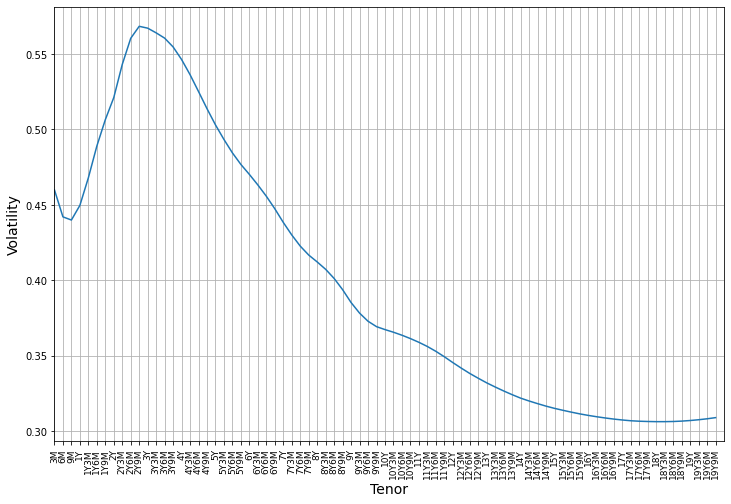
\includegraphics[width=0.5\linewidth]{cap_vola}
	\end{center}
\end{frame}

\begin{frame}{Remarks on LFM and Cap Pricing}
	\begin{itemize}
	\item<1-> A possible explanation is obtained by segmenting the caplet market across three maturities, see (Rebonato, 2002)
	\begin{enumerate} 
	\item<2-> \textbf{Very short end of the curve}: central banks nowadays clearly communicate their strategy so that their actions are by and large anticipated, leading to low volatilities in this region;
	\item<3-> \textbf{6M to 12-18M}: market participants continuously assess their expectations of future monetary policy and also disagree to a large extent on the monetary course in
	the intermediate term;
	\item<4-> \textbf{Longer maturities}: lastly, the third segment is much more affected by structural, long-term
	changes in expectations related to inflation and real rates/real returns. Thus, these long-term concerns are more or less independent of short-term monetary policies and the forward rate volatility is relatively low at the long end of the curve.
	\end{enumerate}	
	\end{itemize}
\end{frame}

\subsection{Log-normal Swap Model}
\begin{frame}{A Model for Swaptions}
  \begin{itemize}
  \item<1-> The counterpart of the Log-normal Forward LIBOR model among the market models, is the \textcolor{red}{Log-normal Forward-Swap Model (LSM)}.
  \item<2-> It describes the evolution of the forward swap rates instead of the forward LIBOR rates, these two kind of rates being the bases of the two main markets in the interest rate derivatives world. 
  \item<3-> The settings of this model are similar to the LFM, the relevant exception being the choice of the more convenient numeraire.
  \end{itemize}
\end{frame}

\begin{frame}{Choice of the Numeraire}
	\begin{itemize}
		\item<1-> From the pricing formula of a payer swaption
		\begin{equation*}
			\textbf{PSw}=\mathbb{E}^{\mathcal{Q}}\left[D(t,T_\alpha)A\max(S_{\alpha,\beta}(T_\alpha)-K, 0)\right]
		\end{equation*}
		it comes clearly that the natural choice of numeraire to model the dynamics of the forward swap rate is
		\begin{equation*}
			A := \sum^\beta_{i=\alpha+1}\tau_i P(t, T_i)
		\end{equation*}
		which is referred to as the \textcolor{red}{annuity} or the \textcolor{red}{present value of a basis point}, given $\alpha, \beta \in \{0,\ldots, M\}, \alpha < \beta$. 
	  \item<2-> Moreover it has the representation of the value at a time $t$ of a traded asset that is a buy-and-hold portfolio consisting, for each $i$, of $\tau_i$ units of the zero coupon bond maturing at $T_i$, thus it is a plausible numeraire.
	\end{itemize}
\end{frame}

\begin{frame}{Choice of the Numeraire}
  \begin{itemize}
  \item<1-> Denoted by $\mathcal{Q}_{\alpha,\beta}$ the EMM associated with the numeraire $A$, the forward swap rate process $S_{\alpha,\beta}$ is a martingale under $\mathcal{Q}_{\alpha,\beta}$, on the interval $[t, T_\alpha]$.
  \begin{equation*}
  	S_{\alpha,\beta}(t) = \cfrac{P(t,T_\alpha)-P(t,T_\beta)}{\sum_{i=\alpha+1}^{\beta}\tau_iP(t,T_i)}
  \end{equation*}
  \item<2-> The probability measure $\mathcal{Q}^{\alpha,\beta}$ is called \textcolor{red}{the (forward) swap measure} related to $\alpha, \beta$.
  \item<2-> We may note that the annuity plays for the swap rate the same role as the zero coupon bond prices did for the forward rates in the LFM. 
  \end{itemize}
\end{frame}

\begin{frame}{Log-normal Forward Swap Model}
  \begin{block}{Definition}
    Consider a fixed subset $T$ of all the pairs of integer indices ($\alpha, \beta$) of the resettlement dates in the tenor structure $\{T_0, T_1,\ldots, T_M\}$ such that $0 \leq \alpha < \beta \leq M$ and consider for each pair a deterministic function of time $t\rightarrow \sigma_{\alpha,\beta}(t)$. A swap market model (LSM) with volatilities $\sigma_{\alpha,\beta}$ assumes that the forward swap rates have the following dynamics under their associated swap measures:
    \begin{equation}
      dS_{\alpha,\beta}(t) = \sigma_{\alpha,\beta}(t)S_{\alpha,\beta}(t)dW_{\alpha,\beta}(t),\quad t \leq T_\alpha
    \end{equation}
    for $(\alpha, \beta) \in T$ pairs, where $W_{\alpha,\beta}$ is a scalar standard $\mathcal{Q}^{\alpha,\beta}$-Brownian motion.
  \end{block}
\end{frame}
%%%We can also allows for correlation between the different Brownian motions, however, this will not affect the swaption prices but only the pricing of more complicated products.
%%
%%%Remark 3. In a model with M + 1 resettlement dates it is possible to model
%%%only M swap rates as independent. The two typical choices of possible T
%%%pairs
%%%identify the following substructures:
%%%• the regular SMM, which models the swap rates S0,M, S1,M, . . . , SM−1,M,
%%%i.e.
%%%T
%%%pairs = {(0, M),(1, M), . . . ,(M − 1, M)} ;
%%%• the reverse SMM, which models the swap rates S0,1, S0,2, . . . , S0,M, i.e.
%%%T
%%%pairs = {(0, 1),(0, 2), . . .,(0, M)} .

\begin{frame}{Equivalence between LSM and Black’s Swaption Prices}
  \begin{block}{Proposition}
    The price of a payer swaption implied by the swap market model coincides with that given by the corresponding Black swaptions formula:
    \begin{equation}
      \textbf{PSw}^{LSM}(0,T_\alpha, [T_\alpha,\ldots,T_\beta],K,v_{\alpha,\beta}(T_\alpha))=
      C_{\alpha, \beta}(0) Bl(K,S_{\alpha,\beta}(0),\sqrt{T_\alpha}v_{\alpha,\beta}(T_\alpha))
      \label{eq:black_swaptions}
    \end{equation}
    where 
	\begin{equation*}    	 
   		v_{\alpha,\beta}^2(T) =\frac{1}{T_\alpha}\int_0^T\sigma_{\alpha,\beta}(t)^2dt 	
    \end{equation*}
  \end{block}
\end{frame}

\subsection{Incompatibility between LFM and LSM}
\begin{frame}{Incompatibility between LFM and LSM}
  A crucial question rises: \textcolor{red}{are the two main Market Models, theoretically consistent ?} 
  Can the assumptions of log-normality of both LIBOR forward rates and forward swap rates coexist? 
  \pause
  In order to give an answer we can proceed as follows:
  \begin{enumerate}
  \item<2-> assume the hypothesis of the LFM, namely that each forward rate $F_i$ is log-normal under its related forward measure $\mathcal{Q}^i$;
  \item<3-> apply the change of measure to obtain their dynamics under the swap measure $\mathcal{Q}^{\alpha,\beta}$, for a choice of $(\alpha,\beta) \in T$ pairs;
  \item<4-> apply the It$\hat{o}$’s formula to obtain the resulting dynamics for the swap rate $S_{\alpha,\beta}$ under $\mathcal{Q}^{\alpha,\beta}$;
  \item<5-> check if this distribution is log-normal, as it is under the hypothesis of the LSM.
  \end{enumerate}
	\uncover<6->{
  \textcolor{red}{Unfortunately, the answer is negative}.} 
\end{frame}

\begin{frame}{Incompatibility between LFM and LSM}
  \begin{itemize}
  \item<1-> However, from a practical point of view, this incompatibility seems to weaken considerably. 
  \item<2-> Indeed, simulating a large number of realizations of $S_{\alpha,\beta}(T_\alpha)$ with the dynamics induced by the LFM one can compute its numerical density and compare it with the log-normal density. 
  \begin{center}
  	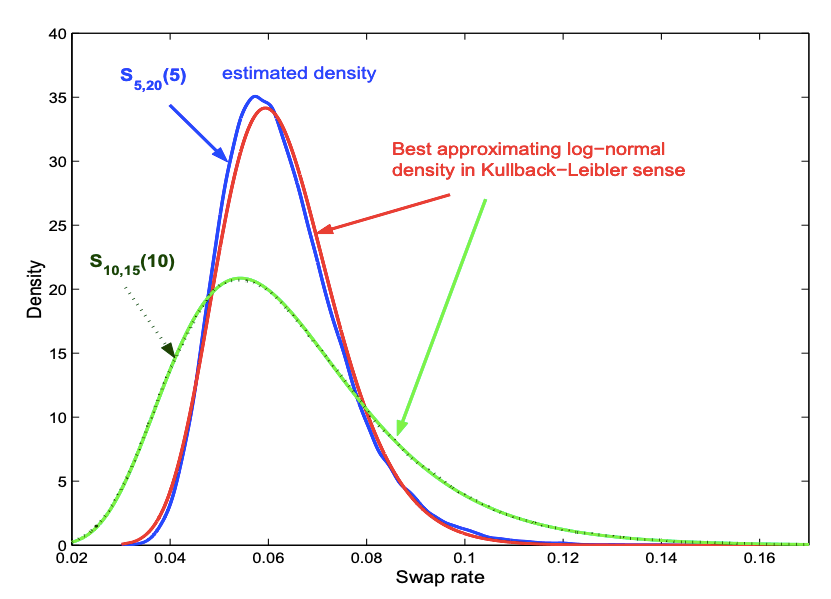
\includegraphics[width=0.45\linewidth]{swap_rate_LFM}
  \end{center}
  \end{itemize}
\end{frame}

\begin{frame}{Incompatibility between LFM and LSM}
	\begin{itemize}
	\item<1-> Consequently, it has been argued that, in normal market conditions, the two distributions are hardly distinguishable.
	\item<2-> Once ascertained the mathematical inconsistency of these two models, we must admit that the LSM is particularly convenient when pricing a swaption, because it yields the practice Black’s formula for swaptions. However, for different products, even those involving the swap rate, there is no analytical formula in general. 
  \item<3-> The problem left is choosing either of the two models for the whole market. After that choice, the half market consistent with the model is calibrated almost automatically, thanks to Black’s formulas, but the remaining half is more intricate to calibrate.
	\end{itemize}
\end{frame}

\begin{frame}{Proposed Solution}
  \begin{itemize}
  \item<1-> Since the LIBOR forward rates, rather than swap rates, are more natural and representative coordinates of the yield curve usually considered, besides being mathematically more manageable, the better choice of modeling may be to assume as framework the LIBOR market model. 
  \item<2-> Thus, hereafter, \textcolor{red}{we are working under the hypothesis of the LFM}.
  %\item The market quotes swaption prices as Black’76 swaption volatilities such that, when inserted into the Black’76 swaption formula, they give the option premium. 
  \item<3-> If we choose one of the discount bonds $P(t, T_i)$ as a numeraire, one forward rate will be a martingale, however, the swap rate being a combination of several forward rates, will not. 
  \item<4-> We thus conclude that swaption pricing via Black’s formula is not possible in the LFM.
    \end{itemize}
\end{frame}

\begin{frame}{Proposed Solution}
	\begin{itemize}
  \item<1-> Brigo and Mercurio derived a complex expression for the swap rate dynamics under the $T$-forward measure induced by the numeraire $P(t, T_i)$.
  \item<2-> But it is not much manageable. There exist, however, very good approximate formulas to the swaption volatility which can be directly used to calibrate to a matrix of quoted swaption volatilities.  
  \item<3-> Also, \textcolor{red}{performing a Monte Carlo simulation to obtain the swaption price is anyway feasible.} 
  
  %\item The LFM, unfortunately, does not feature a known distribution for the joint dynamics of forward rates: to evaluate swaptions, \textcolor{red}{we have to resort to Monte Carlo simulation.}
  \end{itemize}
\end{frame}

\section{Monte Carlo Pricing}
\begin{frame}{Monte Carlo Methods}
  \begin{itemize}
  \item<1-> The Monte Carlo (MC) method is a numerical and probabilistic technique which consists in a computational algorithm relying on repeated independent random sampling to compute approximations of theoretical results.
  \item<2-> In general, MC intends to estimate an expectation value through an arithmetic mean of realizations of i.i.d. random variables and it proceed as follows: 
    \begin{enumerate}
    \item let $X$ be the r.v., with known distribution, on which the expectation we need to estimate depends;
    \item a pseudo-random number generator provides a sequence of realizations $X(k)$ of theoretical independent r.v. $X_1, X_2,\ldots$ distributed as $X$;
    \item then, the desired expectation is approximated by
      \begin{equation*}
	\mathbb{E}[\phi(X)] \approx \frac{1}{m}\sum_{k=1}^m\phi(X^k)
      \end{equation*}
    \end{enumerate}
  \item<3-> Indeed, by the \textcolor{red}{Law of large numbers}, the sample average converges to the expected value, under the hypothesis that $X_i$ is an infinite sequence of i.i.d. random variables with finite expected value.
  \end{itemize}
\end{frame}

\begin{frame}{Monte Carlo Pricing of Swaptions}
  \begin{itemize}
  \item<1-> The most general way to price a swaption, as well as any other option with underlying forward rates, is through Monte Carlo simulation. 
  \item<2-> In order to simulate all the processes involved in the payoff, their joint dynamics is discretized with a numerical scheme for SDEs, e.g. the Euler scheme.
  \item<3-> Recall the price of a payer swaption:
    \begin{equation*}
      \begin{aligned}
        \textbf{PSw} = \mathbb{E}^\mathcal{Q}&\left[D(0, T_\alpha) (S_{\alpha,\beta}(T_\alpha) - K)^+ \sum_{i=\alpha+1}^\beta \tau_i P(T_\alpha, T_i)\right] \\
        &= P(0, T_\alpha)\mathbb{E}^\alpha\left[(S_{\alpha, \beta}(T_\alpha) - K)^+ \sum^\beta_{i=\alpha+1} \tau_i P(T_\alpha, T_i)\right]
      \end{aligned}
    \end{equation*}
    by considering this time $P(\cdot, T_\alpha)$ as numeraire.
  \end{itemize}
\end{frame}

\begin{frame}{Monte Carlo Pricing of Swaptions}
  \begin{itemize}
  \item<1-> Keep in mind that $S_{\alpha,\beta}$ has an expression in terms of the relevant spanning forward rates, and notice that the expectation above depends on the joint distribution of the same $F$’s.
  \item<2-> The dynamics of the $k$-th forward rate, for each $k = \alpha + 1,\ldots, \beta$, under $\mathcal{Q}^\alpha$ is (\cref{eq:forward_rat_dynamics_lfm})
\begin{equation}
  dF_k(t) = \sigma_kF_k\sum_{j=\alpha+1}^k\frac{\rho_{kj}\tau_j\sigma_jF_j}{1+\tau_jF_j}dt+\sigma_kF_k dW^\alpha_k, \quad t<T_\alpha
  \label{eq:dynamics_4.1}
\end{equation}
and, in order to evaluate the swaption payoff we have to generate a number of realization of $F_{\alpha+1}(T_\alpha),\ldots, F_\beta(T_\alpha)$. 
\item<3-> Finally the Monte Carlo price of the swaption is given by the mean of all the payoff evaluations.
  \end{itemize}
\end{frame}

\begin{frame}{Monte Carlo Pricing of Swaptions}
  \begin{itemize}
  \item<1-> Dynamics of \cref{eq:dynamics_4.1} has neither analytical solution nor known distribution, so we need to use the Euler scheme (actually the log version which is easier to handle).
  \item<2-> By the It$\hat{o}$’s formula,
    \begin{equation*}
      d\log F_k(t) = \left(\sigma_k\sum_{j=\alpha+1}^k\frac{\rho_{kj}\tau_j\sigma_jF_j}{1+\tau_jF_j}-\frac{\sigma_k^2}{2}\right)dt+\sigma_k dW^\alpha_k
    \end{equation*}
  \item<3-> Choosing a time grid with step $\Delta t = \cfrac{T_\alpha}{N}$ we get
    \begin{equation*}
      \begin{aligned}
        \log F_k(t_{i+1}) &=\log F_k(t_i) \left(\sigma_k(t_i)\sum_{j=\alpha+1}^k\frac{\rho_{kj}\tau_j\sigma_j(t_i)F_j(t_i)}{1+\tau_jF_j(t_i)}-\frac{\sigma_k(t_i)^2}{2}\right)\Delta t + \\
        &+\sigma_k(t_i) (W^\alpha_k(t_{i+1}) - W^\alpha_k(t_i))
      \end{aligned}
    \end{equation*}
  \item<4-> Which provides us with approximated realizations of the true process $F_k(T_\alpha)$.
  \end{itemize}
\end{frame}

%%Remark 4. We may consider a more refined scheme coming from (4.4) by the
%%following substitution, in the vector version:
%%Σ(ti)(Z
%%α
%%(ti+1) − Z
%%α
%%(ti)) 7−→ ∆ζ(ti),
%%where
%%Σ(t) :=
%%
%%
%%σα+1 0 · · · 0
%%0 σα+2 0 · · · 0
%%.
%%.
%%. 0 .
%%.
%%. 0
%%0 · · · 0 σβ
%%
%%
%%, Zα =
%%
%%
%%Z
%%α
%%α+1
%%Z
%%α
%%α+2
%%.
%%.
%%.
%%Z
%%α
%%β
%%
%%
%%.
%%∆ζ(t) := Z t+∆t
%%t
%%Σ(s)dZα
%%(s) ∼ N (0, Cov(t)),
%%with the covariance n × n matrix, n := β − α, having the elements
%%Covi,j (t) := Z t+∆t
%%t
%%(ΣρΣ
%%′
%%)i,j ds .
%%Indeed, integrating the ln-dynamics (4.3) in the vector version between t
%%and t + ∆t, the resulting stochastic integral in it is just ∆ζ(ti). By means
%%of this substitution, we can simulate more accurate random shocks with
%%gaussian distribution
%%N (0, Cov(t))
%%instead of
%%N (0, ∆tΣρΣ
%%′

\subsection{Confidence Interval}
\begin{frame}{Confidence Interval}
  \begin{itemize}
  \item<1-> Consider a general payoff at time $T$, $\Pi(T)$, depending on a vector of spanning forward LIBOR rates $\bar{F}(t)$. %, for $t \in [0, T]$, where typically $T$ is smaller than or equal to the expiry of the first forward rate.
  \item<2-> We simulate various scenarios of $\Pi(T)$ under the $T$-forward measure. Let $m$ be the number of simulated paths, the Monte Carlo price of the payoff is
    \begin{equation*}
      \mathbb{E}^\mathcal{Q}[D(0,T)\Pi(T)] = P(0,T)\mathbb{E}^T[\Pi(T)]\approx \frac{P(0,T)}{m}\sum_{j=1}^{m}\Pi^j(T)
    \end{equation*}
  \item<3-> Since $\Pi^1(T), \Pi^2(T),\ldots$ is a sequence of realizations of i.i.d. random variables distributed as $\Pi(T)$, the \textcolor{red}{Central Limit Theorem} tell us that for $m\rightarrow\infty$
    \begin{equation*}
      \cfrac{\sum_{j=1}^{m}\Pi^j(T)-\mathbb{E}^T[\Pi(T)]}{\sqrt{m} Std(\Pi(T))}\rightarrow \mathcal{N}(0,1)
    \end{equation*}
  \end{itemize}
\end{frame}

\begin{frame}{Confidence Interval}
  \begin{itemize}
  \item<1-> Thus, for large $m$, the following approximation holds
    \begin{equation*}
      \frac{\sum_{j=1}^{m}\Pi^j}{m}-\mathbb{E}^T[\Pi]\approx \frac{Std(\Pi)}{\sqrt{m}}\mathcal{N}(0,1)
    \end{equation*}
  \item<2-> The probability that the MC estimate is closer than $\epsilon$ to the true price is
    \begin{equation*}
      P\left(\bigg|\frac{\sum_{j=1}^m\Pi^j}{m}-\mathbb{E}^T[\Pi]\bigg|<\epsilon\right) = P\left(|\mathcal{N}(0,1)|<\epsilon\frac{\sqrt{m}}{Std(\Pi)}\right) =
      2\Phi\left(\epsilon\frac{\sqrt{m}}{Std(\Pi)}\right)-1
    \end{equation*}
    where $\Phi$ denotes the c.d.f. of the standard gaussian distribution.
  \end{itemize}
\end{frame}

\begin{frame}{Confidence Interval}
  \begin{columns}
    \column{0.6\linewidth}
    \begin{itemize}
    \item Once we have chosen the desired value for such a probability, we can find the corresponding value for $\epsilon$. For a typical choice of accuracy of 98\%: $\epsilon \approx 2.33 \cfrac{Std(\Pi)}{\sqrt{m}}$
    \item Notice that as $m$ increases, the window shrinks as $1/\sqrt{m}$.
    \end{itemize}
    \column{0.4\linewidth}
    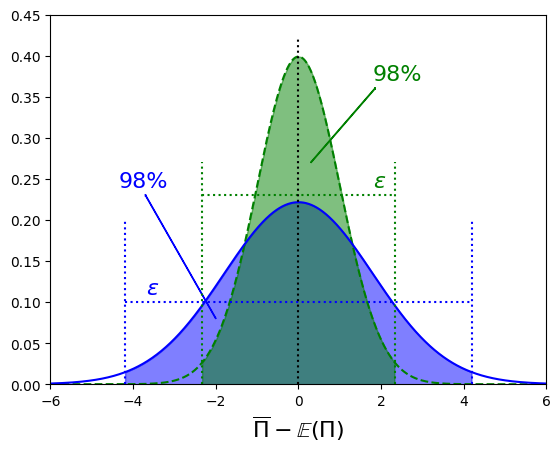
\includegraphics[width=0.9\linewidth]{confidence_interval}
  \end{columns}
  \begin{tikzpicture}[remember picture,overlay]
    \node[xshift=5cm,yshift=-3.7cm] (image) at (current page.center) {
\includegraphics[width=20px]{python_logo}};
    \node[align = center, yshift=1.45cm, below=of image] {\tiny{\href{shorturl.at/NPQT1}{shorturl.at/NPQT1}}};
  \end{tikzpicture}
\end{frame}

\subsection{Variance Reduction}
\begin{frame}{Monte Carlo Variance Reduction}
  To reduce the confidence interval without running too many simulations, i.e. reduce the sample variance, without increasing $m$, the \textcolor{red}{control variate technique} can be used.
  \pause]
  \begin{enumerate}
  \item<2-> Consider another payoff $\Pi_{an}$ which we can be evaluated analytically, whose expectation is denoted by $\mathbb{E}[\Pi_{an}] = \pi_{an}$, and simulate it together with $\Pi$ under the same scenarios for $\bar{F}$.
  \item<3-> Define an unbiased estimator for $\mathbb{E}[\Pi]$ as the sample mean of the r.v. 
    \begin{equation*}
      \Pi_c(\gamma) = \Pi + \gamma(\Pi_{an} - \pi_{an})
    \end{equation*}
    Hence $\Pi_c(\gamma)$ has expectation $\mathbb{E}[\Pi]$ and variance
    \begin{equation*}
      Var(\Pi_c(\gamma)) = Var(\Pi) + \gamma^2 Var(\Pi_{an}) + 2\gamma Cov(\Pi, \Pi_{an})
    \end{equation*}
  \end{enumerate}
\end{frame}

\begin{frame}{Monte Carlo Variance Reduction}
	\begin{enumerate}\addtocounter{enumi}{2}
	\item This can be minimized by choosing the appropriate $\gamma$
	\begin{equation*}
	\gamma^* = -\frac{Cov(\Pi, \Pi_{an})}{Var(\Pi_{an})} = -\frac{Corr(\Pi, \Pi_{an})}{Std(\Pi)Std(\Pi_{an})}, \quad (Corr_{XY}=\frac{Cov_{XY}}{Std_X Std_Y})
	\end{equation*}
  	and the minimum variance of $\Pi_c$ is computed as
    \begin{equation*}
     Var(\Pi_c(\gamma^*)) = Var(\Pi)(1 - Corr(\Pi, \Pi_{an})^2)
    \end{equation*}
    that is \textcolor{red}{smaller than the variance of $\Pi$}. Moreover, the larger the correlation between $\Pi$ and $\Pi_{an}$ the larger the difference between the two variances.
  \end{enumerate}
\end{frame}

\begin{frame}{Monte Carlo Variance Reduction}
	\begin{enumerate}\addtocounter{enumi}{3}
  \item<1-> Moving to the standard deviation
	\begin{equation*}
		Std(\Pi_c(\gamma^*)) = Std(\Pi) \sqrt{(1 - Corr(\Pi, \Pi_{an})^2)}
	\end{equation*}
	the variance reduction will increase with the correlation between $\Pi$ and $\Pi_{an}$. 
	\item<2-> Now if we consider the confidence interval for $\Pi_c$ 
	\begin{equation*}
		98\% C.L. =\left[\Pi_c(\gamma,m) - 2.33\cdot\frac{Std(\Pi_c)}{\sqrt{m}};\Pi_c(\gamma,m) + 2.33\cdot\frac{Std(\Pi_c)}{\sqrt{m}}\right] 
	\end{equation*}
	we get a narrower width by a factor of
	\begin{equation*}
		\sqrt{1 - Corr(\Pi, \Pi_{an}; m)^2}
	\end{equation*}
	\end{enumerate}
\end{frame}

\begin{frame}{Monte Carlo Variance Reduction}
  \begin{itemize}
  \item<1-> This technique is quite general and the choice of $\Pi_{an}$ is theoretically free.
  \item<2-> In the case of the pricing of swaptions in the LFM, we select as $\Pi_{an}$ one of the simplest payoff with underlying rates $F_{\alpha+1},\ldots,F_\beta$, as may be a portfolio of FRA contracts at time $T_\alpha$ on each single time interval $(T_{i-1}, T_i]$.
  \item<3-> Consider the payoff of such portfolio where the $K = F_i(0)$ and rewrite it by a change of measure as follows:
    \begin{equation*}
      \begin{aligned}
        \textbf{FRAs} = &\mathbb{E}^\mathcal{Q}\left[D(0,T_\alpha)\sum_{i=\alpha+1}^\beta P(T_\alpha,T_i)\tau_i(F_i(T_\alpha) - F_i(0))\right] = \\
        &=\mathbb{E}^j\left[\frac{P(0,T_i)}{P(T_\alpha,T_j)}\sum_{i=\alpha+1}^\beta P(T_\alpha,T_i)\tau_i(F_i(T_\alpha) - F_i(0))\right] = \\
        & = P(0,T_j)\mathbb{E}^j\left[\frac{\sum_{i=\alpha+1}^\beta P(T_\alpha,T_i)\tau_i(F_i(T_\alpha) - F_i(0))}{P(T_\alpha,T_j)}\right]
      \end{aligned}
    \end{equation*}
  \end{itemize}
\end{frame}

\begin{frame}{Monte Carlo Variance Reduction}
  \begin{itemize}
  \item<1-> Thus we can set
    \begin{equation*}
      \Pi_{an}(T_\alpha) = \frac{\sum_{i=\alpha+1}^\beta P(T_\alpha,T_i)\tau_i(F_i(T_\alpha) - F_i(0))}{P(T_\alpha,T_j)}
    \end{equation*}
    whose price at time 0 is $\pi_{an} = 0$.
  \item<2-> Indeed, the payoff $\Pi_{an}(\cdot)$ is a sum of traded assets divided by $P(\cdot, T_j)$, hence it is a martingale under the $T^j$-forward measure $\mathcal{Q}^j$, which implies that
    
    \begin{equation*}
      \mathbb{E}^j[\Pi_{an}(T_\alpha)] = \mathbb{E}^j[\Pi_{an}(0)] = 0
    \end{equation*}
  \end{itemize}
\end{frame}

\section{Correlated Brownian Motions}
\subsection{Decorrelation}
\begin{frame}{Correlated Brownian Motions}
  \begin{itemize}
  \item<1-> Correlation is a linear measure of dependency between random variables. Given two random variables $X$ and $Y$, it is given by
  	\begin{equation*}
  		\rho_{X,Y} = \frac{\mathbb{E}((X-\mathbb{E}(X))(Y-\mathbb{E}(Y))}{\sigma_X \sigma_Y}
  	\end{equation*}
  \item<2-> In the LFM, we can assume that the Brownian motions driving the dynamics of forward rate are correlated
    \begin{equation}
      <dW_t^{T_i}, dW_t^{T_i}> = \rho_{ij}dt
    \end{equation}
  \item<3-> This model feature is included because the value of a swaption at maturity is influenced by the joint distribution of forward rates and thus by the correlation amongst them. 
  \item<4-> Since the underlying in a swaption is a swap rate which in turn is a weighted average of forward rates, we expect the price of a swaption to increase if the forward rates become more correlated. 
  \end{itemize}
\end{frame}

\begin{frame}{Correlated Brownian Motions}
	\begin{itemize}
		\item In models for short rate it is assumed full correlation $\rho_{ij}=1$, which is a tight constraint on the dynamics of the forward rates.
		\item In the LFM, we can allow \textcolor{red}{decorrelation} to better fit the derivatives at hand
		\begin{equation*}
			dF_k(t) = \sigma_kF_k\sum_{j=\alpha+1}^k\frac{\boxed{\rho_{kj}}\tau_j\sigma_jF_j}{1+\tau_jF_j}dt+\sigma_kF_k dZ^\alpha_k
		\end{equation*}
	\end{itemize}
\end{frame}

\begin{frame}{Instantaneous and Terminal Correlation}
	%\begin{itemize}
	%\item For calibrating a LIBOR market model, instantaneous
	%  correlation is modeled. However, for pricing correlation-sensitive products, terminal correlation is used.
	%\item Define an $n$-dimensional LFM with $m$ factors:
	%\begin{equation*}
	%	\frac{df_i}{f_i} = \mu_i dt + \sigma_i \sum_{k=1}^m b_{ik}dZ_k
	%\end{equation*}
	%with $b_k=\frac{\sigma_{ik}}{\sqrt{\sum_{k=1}^m\sigma_{ik}^2}}$
	
	\begin{block}{Definition}
		The \textcolor{red}{instantaneous correlation} is a quantity summarizing the degree of “dependence” between changes of different forward rates.
		\begin{equation*}
			\rho_{ij} = \frac{dF_i(t) dF_j(t)}{Std(dF_i(t)) Std(dF_j(t))}
		\end{equation*}
		%where $Std$ denotes the standard deviation conditional on the information available at time $t$ at which the change occurs. 
		%The instantaneous correlation of the LIBOR rates $L(t, T_{i-1}, T_i)$ and $L(t, T_{j-1}, T_j)$ is given by the correlation of the increments of the Brownian motions:
		%\begin{equation*}
		%\rho_{i,j}(t) = \sum_{k=1}^m b_{i,k}b_{j,k}, \quad i,j=1,\ldots,n
		%\end{equation*}
		%From this formula it is clear that indeed the instantaneous correlation ρ is related to changes dF in for- ward rates. Instead, 
		The \textcolor{red}{terminal correlation} is a quantity summarizing the degree of “dependence” between two different forward rates at a given \emph{terminal} time-instant. Typically, the $T_1$ terminal correlation between $F_i$ and $F_j$ is the correlation between $F_i(T_1)$ and $F_j(T_1)$.
	\end{block}
	It is important to understand how instantaneous correlation in the forward-rate dynamics translates into a terminal correlation of simple rates.
	%\begin{block}{Definition}
	%The terminal correlation of the LIBOR rates$L(t, T_{i-1}, T_i)$ and $L(t, T_{j-1}, T_j)$ is given by
	%\begin{equation*}
	%\tilde{\rho}_{i,j}(t) = %\frac{\int_o^t\sigma_i(u)\sigma_j(u)\rho_{i,j}(u)du}{\sqrt{\int_0^t\sigma_i(u)^2du\int_o^t\sigma_j(u)^2du}}
	%\end{equation*}
	%\end{block}
	%\end{itemize}
\end{frame}

\begin{frame}{Instantaneous Correlation}
  \begin{itemize}    
  \item<1-> Insantaneous correlation can be estimated from historical market data.
  \begin{enumerate}
	  \item first derive yield curves for some period of time in the past;
	  \item then, forward curves may be calculated off the yield curves;
	  \item finally the dependence between forward rate increments may be estimated. 
  \end{enumerate}
  \item<2-> Anyway it would be nice to imply these correlations out of liquidly traded swaption prices. 
  \item<3-> Many parametrizations functions have been introduced to express a given correlation matrix of forward rates in a functional form.
  \item<4-> This has several advantages: it is computationally convenient to work with an analytical formula. Noise (e.g. non-synchronous data or illiquidity) is removed by focussing on general properties of correlation. Furthermore, the correlation matrix rank can be controlled through the functional form.
  \end{itemize}
\end{frame}

\begin{frame}{Correlation Parametrization}
  \begin{itemize}
  \item One property that is always implicitly present is time-homogeneity: correlation of forward rates does not depend on calendar time $t$, but only on the rates’ time to maturity $T_i-t$.
  %\item An important aspect of these parameterizations is the number of parameters used to fit the market data. Most parameterizations advocate the use of few parameters that emphasize general properties of market correlation and prevent overfitting.
  \item General requirements on an $M \times M$ correlation matrix $\rho$ are:
	\begin{enumerate}
		\item $\rho$ must be real and symmetric;
		\item $\rho_{i,i}=1$ for $i = 1,\ldots, M$;
		\item $\rho$ must be positive semi-definite such that can be decomposed into $\rho = BB^T$.
	\end{enumerate}
	\item Usually parameterizations are determined by minimizing the mean square error between historical market correlation and parameterized functional form.
	\end{itemize}
\end{frame}

\begin{frame}{Decorrelation}
\begin{itemize}
	\item<1-> Generally, inferring instantaneous correlations from actively traded swaptions is desirable as they reflect current market conditions, thus not suffering from the backward-looking nature of historically estimated correlations. 
	\item<2-> There are however, also problems with implying correlations from the market. One such general problem is that swaption prices depend on forward rate correlation AND volatility. 
	\item<3-> There is no liquidly traded fixed income derivative that solely depends on correlation, as opposed to caplets, which solely depend on volatility.
	\item<4-> Another problem concerns the relationship between instantaneous and terminal correlations.
\end{itemize}
\end{frame}	
	 
\begin{frame}{Decorrelation}
	\begin{itemize}
	\item<1-> For terminal correlations, (Rebonato, 1998) shows that the appropriate quantity summarizing the amount of decorrelation between two stochastic variables from time 0 to time $T$ is
	\begin{equation}		
		\tilde{\rho}_{ij}(t)=\frac{\int_0^t\sigma_i(u)\sigma_j(u)\rho_{ij}(u)du}{\sqrt{\int_0^t\sigma_i(u)^2 du\int_0^t\sigma_j(u)^2 du}}	
		\label{eq:terminal_correlation}
	\end{equation}
	\item<2-> From this equation, we see that the terminal correlation not only depends on the instantaneous correlation $\rho_{ij}$ but also on the instantaneous volatilities. Hence, even for perfectly instantaneously correlated random variables, $\rho_{ij}= 1$, terminal \textcolor{red}{decorrelation} could be achieved by time-dependent instantaneous volatilities.
\end{itemize}
\end{frame}	
%  \begin{itemize}
%  \item Is terminal correlation completely determined by the instantaneous correlations $\rho_{ij}$ between $W_i$ and $W_j$ ?
%  \item The answer is no, since terminal correlation also depends on the forward rate volatilities (caplet volatilities). 
%  \item In particular it is important the choice of the function $\sigma(t)$ used to recover "average volatilities" through integration in $[0,T_i]$.
%  \item If \textcolor{red}{instantaneous volatilities} are not constant, they have a significant impact on terminal correlation and can produce terminal \emph{decorrelation}, even in the case of perfect instantaneous correlation.
%  %\item Prices of correlation-sensitive products depend on terminal correlation, and thus instantaneous correlation and instantaneous volatility. 
%  %\item It is important to note that there is no instrument that is sensitive solely to instantaneous correlation. Therefore, estimating correlation from a product that is sensitive to multiple factors is not straight-forward and can lead to ambiguous results.
%  \end{itemize}
%\end{frame}

\begin{frame}{An Example}
\begin{itemize}
	\item<1-> Considering Rebonato's analytical formula for terminal correlation \cref{eq:terminal_correlation}it can be shown that in the case of piecewise-constant volatilities, terminal correlation is just the average correlation over the period. 
  	\item<2-> Since the instantaneous volatilities are constant, they can be factored out from the integrals
	  \begin{equation*}	    \tilde{\rho}_{ij}(t)=\frac{\cancel{\sigma_i}\cancel{\sigma_j}\int_0^t\rho_{ij}(u)du}{\sqrt{\cancel{\sigma_i^2}\cancel{\sigma_j^2} t^2}}= \frac{\int_0^t\rho_{ij}(u)du}{t}		
  	\end{equation*}
  	which indeed leads to lower terminal correlation.
  	\item<3-> Swaption payoffs depend on the terminal correlation between several different forward rates which leads (Brigo and Mercurio, 2006) to the conclusion that swaption volatilities are more directly linked with terminal correlations rather than with instantaneous ones.
  \end{itemize}
\end{frame}

\end{document}
